\documentclass[11pt]{article}
\usepackage[margin=1in]{geometry}
\usepackage{amsmath,amssymb}
\usepackage{graphicx}
\usepackage{booktabs}
\usepackage{array}
\usepackage{longtable}
\usepackage{hyperref}
\usepackage{natbib}
\usepackage{xcolor}
\usepackage{microtype}
\usepackage[affil-it]{authblk}
\usepackage[section]{placeins}

\newcommand{\TODO}[1]{\textcolor{red}{[TODO: #1]}}

% Extra space before floats (matches pQTL/cross-ancestry papers)
\setlength{\textfloatsep}{14pt plus 2pt minus 2pt}
\setlength{\intextsep}{10pt plus 2pt minus 2pt}

\title{The Composition Confound:\\Partner-Specific Base-Pairing Responses Survive Matched\\Controls in Three of Ten Nucleic Acid Language Models}

\author{Elliot Tower}
\affil{Independent researcher \\ \texttt{elliot@elliottower.ai}}
\date{}

% Running head for RNA journal (<=50 chars):
% The composition confound in nucleic acid language models

% Panel counts and every reported number, written by
% scripts/generate_results_tables.py from the stamped runs.
% Generated by scripts/generate_panel_description.py. Do not edit.
% Every figure below is computed from data/rfam_families/.
\newcommand{\panelN}{47}
\newcommand{\panelCurated}{52}
\newcommand{\panelWithdrawn}{5}
\newcommand{\panelClasses}{riboswitches (14), cis-regulatory elements (8), other ncRNAs (8), ribozymes (6), miRNA precursors (4), snRNAs (4), tRNAs (2), and CRISPR repeats (1)}
\newcommand{\panelLengthRange}{30--387}
\newcommand{\panelLengthMedian}{106}
\newcommand{\panelLengthIQR}{77.5--166}
\newcommand{\panelStemGC}{59.1}
\newcommand{\panelLoopGC}{43.0}
\newcommand{\panelGCEnriched}{40}
\newcommand{\panelGCScored}{47}

% Written by scripts/generate_results_tables.py. Do not edit.
\newcommand{\paramsOverEvo}{75}
\newcommand{\paramsOverRiNALMo}{7.5}
\newcommand{\confirmatoryN}{36}
\newcommand{\rungThreeQualifying}{38}
\newcommand{\rungThreeQuarantined}{2}
\newcommand{\chanceRateN}{35}
\newcommand{\chanceRateMin}{0.000}
\newcommand{\chanceRateMax}{0.316}
\newcommand{\gateThreshold}{8}
\newcommand{\gateRegistered}{7}
\newcommand{\bootstrapB}{10{,}000}
\newcommand{\panelHashShort}{\texttt{5c4d6f6d4c32}}
\newcommand{\provenanceRuns}{17}
\newcommand{\provenanceCommits}{2}
\newcommand{\provenanceStacks}{5}
\newcommand{\ratioErnieRNA}{1.276}
\newcommand{\ciErnieRNA}{[1.22, 1.34]}
\newcommand{\exceedErnieRNA}{31}
\newcommand{\dinucErnieRNA}{30}
\newcommand{\retainErnieRNA}{30 of 31}
\newcommand{\retainPctErnieRNA}{97\%}
\newcommand{\probeErnieRNA}{0.683}
\newcommand{\probeDeltaErnieRNA}{+0.183}
\newcommand{\probeLayerErnieRNA}{11}
\newcommand{\attnErnieRNA}{0.113}
\newcommand{\psErnieRNA}{0.1113}
\newcommand{\gateErnieRNA}{34/36}
\newcommand{\gateCountErnieRNA}{34}
\newcommand{\eligibleErnieRNA}{36}
\newcommand{\nullErnieRNA}{32/34}
\newcommand{\consErnieRNA}{32/34}
\newcommand{\hthreeErnieRNA}{0.885}
\newcommand{\psPeakErnieRNA}{12}
\newcommand{\psLayersErnieRNA}{13}
\newcommand{\psPeakCountErnieRNA}{29 of 34}
\newcommand{\ratioRiNALMo}{1.143}
\newcommand{\ciRiNALMo}{[1.12, 1.17]}
\newcommand{\exceedRiNALMo}{17}
\newcommand{\dinucRiNALMo}{15}
\newcommand{\retainRiNALMo}{15 of 17}
\newcommand{\retainPctRiNALMo}{88\%}
\newcommand{\probeRiNALMo}{0.634}
\newcommand{\probeDeltaRiNALMo}{+0.134}
\newcommand{\probeLayerRiNALMo}{32}
\newcommand{\attnRiNALMo}{0.107}
\newcommand{\psRiNALMo}{0.2062}
\newcommand{\gateRiNALMo}{33/36}
\newcommand{\gateCountRiNALMo}{33}
\newcommand{\eligibleRiNALMo}{36}
\newcommand{\nullRiNALMo}{29/33}
\newcommand{\consRiNALMo}{29/33}
\newcommand{\hthreeRiNALMo}{0.859}
\newcommand{\psPeakRiNALMo}{33}
\newcommand{\psLayersRiNALMo}{34}
\newcommand{\psPeakCountRiNALMo}{31 of 33}
\newcommand{\ratioRNAFM}{1.129}
\newcommand{\ciRNAFM}{[1.11, 1.15]}
\newcommand{\exceedRNAFM}{17}
\newcommand{\dinucRNAFM}{14}
\newcommand{\retainRNAFM}{14 of 17}
\newcommand{\retainPctRNAFM}{82\%}
\newcommand{\probeRNAFM}{0.591}
\newcommand{\probeDeltaRNAFM}{+0.091}
\newcommand{\probeLayerRNAFM}{8}
\newcommand{\attnRNAFM}{0.098}
\newcommand{\psRNAFM}{0.0117}
\newcommand{\gateRNAFM}{31/36}
\newcommand{\gateCountRNAFM}{31}
\newcommand{\eligibleRNAFM}{36}
\newcommand{\nullRNAFM}{26/31}
\newcommand{\consRNAFM}{26/31}
\newcommand{\hthreeRNAFM}{0.717}
\newcommand{\psPeakRNAFM}{6}
\newcommand{\psLayersRNAFM}{13}
\newcommand{\psPeakCountRNAFM}{24 of 31}
\newcommand{\ratioUTRLM}{1.056}
\newcommand{\ciUTRLM}{[1.04, 1.08]}
\newcommand{\exceedUTRLM}{3}
\newcommand{\dinucUTRLM}{2}
\newcommand{\retainUTRLM}{2 of 3}
\newcommand{\retainPctUTRLM}{67\%}
\newcommand{\probeUTRLM}{0.578}
\newcommand{\probeDeltaUTRLM}{+0.078}
\newcommand{\probeLayerUTRLM}{1}
\newcommand{\attnUTRLM}{0.051}
\newcommand{\psUTRLM}{$8.3 \times 10^{-6}$}
\newcommand{\gateUTRLM}{13/36}
\newcommand{\gateCountUTRLM}{13}
\newcommand{\eligibleUTRLM}{36}
\newcommand{\nullUTRLM}{4/13}
\newcommand{\consUTRLM}{4/13}
\newcommand{\hthreeUTRLM}{0.345}
\newcommand{\psPeakUTRLM}{4}
\newcommand{\psLayersUTRLM}{7}
\newcommand{\psPeakCountUTRLM}{3 of 13}
\newcommand{\ratioSpliceBERT}{1.040}
\newcommand{\ciSpliceBERT}{[1.03, 1.05]}
\newcommand{\exceedSpliceBERT}{3}
\newcommand{\dinucSpliceBERT}{1}
\newcommand{\retainSpliceBERT}{1 of 3}
\newcommand{\retainPctSpliceBERT}{33\%}
\newcommand{\probeSpliceBERT}{0.566}
\newcommand{\probeDeltaSpliceBERT}{+0.066}
\newcommand{\probeLayerSpliceBERT}{1}
\newcommand{\attnSpliceBERT}{0.054}
\newcommand{\psSpliceBERT}{0.0002}
\newcommand{\gateSpliceBERT}{22/36}
\newcommand{\gateCountSpliceBERT}{22}
\newcommand{\eligibleSpliceBERT}{36}
\newcommand{\nullSpliceBERT}{3/22}
\newcommand{\consSpliceBERT}{3/22}
\newcommand{\hthreeSpliceBERT}{0.290}
\newcommand{\psPeakSpliceBERT}{0}
\newcommand{\psLayersSpliceBERT}{7}
\newcommand{\psPeakCountSpliceBERT}{8 of 22}
\newcommand{\ratioNTvTwo}{1.098}
\newcommand{\ciNTvTwo}{[1.08, 1.12]}
\newcommand{\exceedNTvTwo}{9}
\newcommand{\dinucNTvTwo}{8}
\newcommand{\retainNTvTwo}{8 of 9}
\newcommand{\retainPctNTvTwo}{89\%}
\newcommand{\probeNTvTwo}{0.536}
\newcommand{\probeDeltaNTvTwo}{+0.036}
\newcommand{\probeLayerNTvTwo}{7}
\newcommand{\attnNTvTwo}{0.234}
\newcommand{\psNTvTwo}{$-9.7 \times 10^{-5}$}
\newcommand{\gateNTvTwo}{34/36}
\newcommand{\gateCountNTvTwo}{34}
\newcommand{\eligibleNTvTwo}{36}
\newcommand{\nullNTvTwo}{6/34}
\newcommand{\consNTvTwo}{6/34}
\newcommand{\hthreeNTvTwo}{0.007}
\newcommand{\psPeakNTvTwo}{0}
\newcommand{\psLayersNTvTwo}{13}
\newcommand{\psPeakCountNTvTwo}{27 of 34}
\newcommand{\ratioDNABERTTwo}{0.996}
\newcommand{\ciDNABERTTwo}{[0.98, 1.01]}
\newcommand{\exceedDNABERTTwo}{3}
\newcommand{\dinucDNABERTTwo}{2}
\newcommand{\retainDNABERTTwo}{2 of 3}
\newcommand{\retainPctDNABERTTwo}{67\%}
\newcommand{\probeDNABERTTwo}{0.551}
\newcommand{\probeDeltaDNABERTTwo}{+0.051}
\newcommand{\probeLayerDNABERTTwo}{8}
\newcommand{\attnDNABERTTwo}{0.196}
\newcommand{\psDNABERTTwo}{-0.0180}
\newcommand{\gateDNABERTTwo}{24/36}
\newcommand{\gateCountDNABERTTwo}{24}
\newcommand{\eligibleDNABERTTwo}{36}
\newcommand{\nullDNABERTTwo}{4/24}
\newcommand{\consDNABERTTwo}{4/24}
\newcommand{\hthreeDNABERTTwo}{0.000}
\newcommand{\psPeakDNABERTTwo}{0}
\newcommand{\psLayersDNABERTTwo}{1}
\newcommand{\psPeakCountDNABERTTwo}{24 of 24}
\newcommand{\ratioHyenaDNA}{1.160}
\newcommand{\ciHyenaDNA}{[1.12, 1.20]}
\newcommand{\exceedHyenaDNA}{8}
\newcommand{\dinucHyenaDNA}{7}
\newcommand{\retainHyenaDNA}{7 of 8}
\newcommand{\retainPctHyenaDNA}{88\%}
\newcommand{\probeHyenaDNA}{0.577}
\newcommand{\probeDeltaHyenaDNA}{+0.077}
\newcommand{\probeLayerHyenaDNA}{0}
\newcommand{\psHyenaDNA}{0.0002}
\newcommand{\gateHyenaDNA}{7/36}
\newcommand{\gateCountHyenaDNA}{7}
\newcommand{\eligibleHyenaDNA}{36}
\newcommand{\nullHyenaDNA}{3/7}
\newcommand{\consHyenaDNA}{3/7}
\newcommand{\hthreeHyenaDNA}{0.254}
\newcommand{\psPeakHyenaDNA}{0}
\newcommand{\psLayersHyenaDNA}{4}
\newcommand{\psPeakCountHyenaDNA}{6 of 7}
\newcommand{\ratioCaduceus}{1.206}
\newcommand{\ciCaduceus}{[1.16, 1.26]}
\newcommand{\exceedCaduceus}{8}
\newcommand{\dinucCaduceus}{4}
\newcommand{\retainCaduceus}{4 of 8}
\newcommand{\retainPctCaduceus}{50\%}
\newcommand{\probeCaduceus}{0.577}
\newcommand{\probeDeltaCaduceus}{+0.077}
\newcommand{\probeLayerCaduceus}{0}
\newcommand{\psCaduceus}{0.0039}
\newcommand{\gateCaduceus}{16/36}
\newcommand{\gateCountCaduceus}{16}
\newcommand{\eligibleCaduceus}{36}
\newcommand{\nullCaduceus}{8/16}
\newcommand{\consCaduceus}{8/16}
\newcommand{\hthreeCaduceus}{0.442}
\newcommand{\psPeakCaduceus}{3}
\newcommand{\psLayersCaduceus}{17}
\newcommand{\psPeakCountCaduceus}{4 of 16}
\newcommand{\ratioEvo}{1.458}
\newcommand{\ciEvo}{[1.30, 1.64]}
\newcommand{\exceedEvo}{8}
\newcommand{\dinucEvo}{6}
\newcommand{\retainEvo}{6 of 8}
\newcommand{\retainPctEvo}{75\%}
\newcommand{\probeEvo}{0.552}
\newcommand{\probeDeltaEvo}{+0.052}
\newcommand{\probeLayerEvo}{0}
\newcommand{\psEvo}{0.0017}
\newcommand{\gateEvo}{13/36}
\newcommand{\gateCountEvo}{13}
\newcommand{\eligibleEvo}{36}
\newcommand{\nullEvo}{2/13}
\newcommand{\consEvo}{2/13}
\newcommand{\hthreeEvo}{0.376}
\newcommand{\psPeakEvo}{12}
\newcommand{\psLayersEvo}{32}
\newcommand{\psPeakCountEvo}{7 of 13}
\newcommand{\exceedUntrainedErnieRNA}{10}
\newcommand{\ratioUntrainedErnieRNA}{1.164}
\newcommand{\retainUntrainedErnieRNA}{6 of 10}
\newcommand{\attnUntrainedErnieRNA}{0.085}
\newcommand{\attnDeltaErnieRNA}{+0.027}
\newcommand{\attnFamilyDeltaErnieRNA}{+0.027}
\newcommand{\attnHigherTrainedErnieRNA}{47}
\newcommand{\attnHigherUntrainedErnieRNA}{0}
\newcommand{\psUntrainedErnieRNA}{$3.4 \times 10^{-9}$}
\newcommand{\gateUntrainedErnieRNA}{13/36}
\newcommand{\nullUntrainedErnieRNA}{11/13}
\newcommand{\signErnieRNA}{35/47}
\newcommand{\signPctErnieRNA}{74\%}
\newcommand{\exceedUntrainedRiNALMo}{10}
\newcommand{\ratioUntrainedRiNALMo}{1.156}
\newcommand{\retainUntrainedRiNALMo}{7 of 10}
\newcommand{\attnUntrainedRiNALMo}{0.064}
\newcommand{\attnDeltaRiNALMo}{+0.044}
\newcommand{\attnFamilyDeltaRiNALMo}{+0.044}
\newcommand{\attnHigherTrainedRiNALMo}{46}
\newcommand{\attnHigherUntrainedRiNALMo}{1}
\newcommand{\psUntrainedRiNALMo}{$2.2 \times 10^{-9}$}
\newcommand{\gateUntrainedRiNALMo}{10/36}
\newcommand{\nullUntrainedRiNALMo}{1/10}
\newcommand{\signRiNALMo}{18/47}
\newcommand{\signPctRiNALMo}{38\%}
\newcommand{\exceedUntrainedRNAFM}{1}
\newcommand{\ratioUntrainedRNAFM}{1.045}
\newcommand{\retainUntrainedRNAFM}{1 of 1}
\newcommand{\attnUntrainedRNAFM}{0.038}
\newcommand{\attnDeltaRNAFM}{+0.059}
\newcommand{\attnFamilyDeltaRNAFM}{+0.059}
\newcommand{\attnHigherTrainedRNAFM}{47}
\newcommand{\attnHigherUntrainedRNAFM}{0}
\newcommand{\psUntrainedRNAFM}{$2.0 \times 10^{-10}$}
\newcommand{\gateUntrainedRNAFM}{20/36}
\newcommand{\nullUntrainedRNAFM}{7/20}
\newcommand{\signRNAFM}{43/47}
\newcommand{\signPctRNAFM}{91\%}
\newcommand{\exceedUntrainedUTRLM}{1}
\newcommand{\ratioUntrainedUTRLM}{1.038}
\newcommand{\retainUntrainedUTRLM}{0 of 1}
\newcommand{\attnUntrainedUTRLM}{0.054}
\newcommand{\attnDeltaUTRLM}{-0.003}
\newcommand{\attnFamilyDeltaUTRLM}{-0.003}
\newcommand{\attnHigherTrainedUTRLM}{16}
\newcommand{\attnHigherUntrainedUTRLM}{31}
\newcommand{\psUntrainedUTRLM}{$2.3 \times 10^{-9}$}
\newcommand{\gateUntrainedUTRLM}{28/36}
\newcommand{\nullUntrainedUTRLM}{10/28}
\newcommand{\signUTRLM}{31/47}
\newcommand{\signPctUTRLM}{66\%}
\newcommand{\exceedUntrainedSpliceBERT}{0}
\newcommand{\ratioUntrainedSpliceBERT}{1.054}
\newcommand{\attnUntrainedSpliceBERT}{0.032}
\newcommand{\attnDeltaSpliceBERT}{+0.022}
\newcommand{\attnFamilyDeltaSpliceBERT}{+0.022}
\newcommand{\attnHigherTrainedSpliceBERT}{45}
\newcommand{\attnHigherUntrainedSpliceBERT}{2}
\newcommand{\psUntrainedSpliceBERT}{$6.7 \times 10^{-15}$}
\newcommand{\gateUntrainedSpliceBERT}{11/36}
\newcommand{\nullUntrainedSpliceBERT}{3/11}
\newcommand{\signSpliceBERT}{17/47}
\newcommand{\signPctSpliceBERT}{36\%}
\newcommand{\exceedUntrainedNTvTwo}{5}
\newcommand{\ratioUntrainedNTvTwo}{1.015}
\newcommand{\retainUntrainedNTvTwo}{4 of 5}
\newcommand{\attnUntrainedNTvTwo}{0.241}
\newcommand{\attnDeltaNTvTwo}{-0.007}
\newcommand{\attnFamilyDeltaNTvTwo}{-0.007}
\newcommand{\attnHigherTrainedNTvTwo}{24}
\newcommand{\attnHigherUntrainedNTvTwo}{23}
\newcommand{\psUntrainedNTvTwo}{$-3.4 \times 10^{-5}$}
\newcommand{\gateUntrainedNTvTwo}{33/36}
\newcommand{\nullUntrainedNTvTwo}{9/33}
\newcommand{\signNTvTwo}{43/47}
\newcommand{\signPctNTvTwo}{91\%}
\newcommand{\exceedUntrainedDNABERTTwo}{6}
\newcommand{\ratioUntrainedDNABERTTwo}{33.880}
\newcommand{\retainUntrainedDNABERTTwo}{4 of 6}
\newcommand{\attnUntrainedDNABERTTwo}{0.153}
\newcommand{\attnDeltaDNABERTTwo}{+0.043}
\newcommand{\attnFamilyDeltaDNABERTTwo}{+0.043}
\newcommand{\attnHigherTrainedDNABERTTwo}{37}
\newcommand{\attnHigherUntrainedDNABERTTwo}{10}
\newcommand{\psUntrainedDNABERTTwo}{-0.0003}
\newcommand{\gateUntrainedDNABERTTwo}{19/36}
\newcommand{\nullUntrainedDNABERTTwo}{2/19}
\newcommand{\signDNABERTTwo}{22/47}
\newcommand{\signPctDNABERTTwo}{47\%}
\newcommand{\domainRankBiserial}{+0.52}
\newcommand{\domainP}{0.222}
\newcommand{\familiesScored}{47}
\newcommand{\expectedFalsePositives}{2.4}
\newcommand{\tuPerFamilyRNAFM}{1.08}
\newcommand{\tuOfMeansRNAFM}{1.08}
\newcommand{\tuPerFamilyRiNALMo}{1.00}
\newcommand{\tuOfMeansRiNALMo}{0.99}
\newcommand{\tuPerFamilySpliceBERT}{0.99}
\newcommand{\tuOfMeansSpliceBERT}{0.99}
\newcommand{\transversionAlphabet}{A$\to$C, C$\to$A, G$\to$U, U$\to$C}
\newcommand{\transErnieRNA}{1.253}
\newcommand{\transDeltaErnieRNA}{-1.7\%}
\newcommand{\transRiNALMo}{1.144}
\newcommand{\transDeltaRiNALMo}{+0.1\%}
\newcommand{\transRNAFM}{1.088}
\newcommand{\transDeltaRNAFM}{-3.6\%}
\newcommand{\transUTRLM}{1.058}
\newcommand{\transDeltaUTRLM}{+0.2\%}
\newcommand{\transSpliceBERT}{1.051}
\newcommand{\transDeltaSpliceBERT}{+1.0\%}
\newcommand{\transNTvTwo}{1.109}
\newcommand{\transDeltaNTvTwo}{+1.0\%}
\newcommand{\transDNABERTTwo}{0.995}
\newcommand{\transDeltaDNABERTTwo}{-0.1\%}
\newcommand{\transHyenaDNA}{1.073}
\newcommand{\transDeltaHyenaDNA}{-7.5\%}
\newcommand{\transCaduceus}{1.158}
\newcommand{\transDeltaCaduceus}{-4.0\%}
\newcommand{\transEvo}{1.465}
\newcommand{\transDeltaEvo}{+0.4\%}
\newcommand{\transversionWidest}{HyenaDNA}
\newcommand{\transversionWidestDeviation}{7.5\%}
\newcommand{\transversionBound}{8\%}
\newcommand{\attnBound}{0.05}
\newcommand{\attnWidest}{RNA-FM}
\newcommand{\attnWidestFactor}{2.6}
\newcommand{\psSeparation}{9}

% Written by scripts/generate_arm_tables.py. Do not edit.
\newcommand{\synPSRiNALMo}{0.0919}
\newcommand{\synPSDropRiNALMo}{55\%}
\newcommand{\synExcessRiNALMo}{+0.582}
\newcommand{\natExcessRiNALMo}{+0.770}
\newcommand{\synRetainedRiNALMo}{76\%}
\newcommand{\synPSErnieRNA}{0.0415}
\newcommand{\synPSDropErnieRNA}{63\%}
\newcommand{\synExcessErnieRNA}{+0.574}
\newcommand{\natExcessErnieRNA}{+0.764}
\newcommand{\synRetainedErnieRNA}{75\%}
\newcommand{\synN}{195}
\newcommand{\synPerFamily}{5}
\newcommand{\httModels}{9}
\newcommand{\httHighProbing}{6}
\newcommand{\httHighProbingClean}{6}
\newcommand{\httMonotone}{8}
\newcommand{\multiseqN}{230}
\newcommand{\multiseqFamilies}{47}
\newcommand{\multiseqStable}{8}
\newcommand{\multiseqStableList}{UTR-LM (0.025), SpliceBERT (0.027), RNA-FM (0.034), RiNALMo (0.036), NT~v2 (0.044), DNABERT-2 (0.054), ERNIE-RNA (0.059), Caduceus (0.060)}
\newcommand{\cvRiNALMo}{0.036}
\newcommand{\cvErnieRNA}{0.059}
\newcommand{\cvRNAFM}{0.034}
\newcommand{\cvEvo}{0.180}

% Written by scripts/layer_selection_audit_v2.py. Do not edit.
\newcommand{\selectionDepthRho}{+0.06}
\newcommand{\selectionDepthP}{0.85}
\newcommand{\selectionArms}{13}
\newcommand{\selLayersErnieRNA}{13}
\newcommand{\selChanceErnieRNA}{0.091}
\newcommand{\selChancePanelErnieRNA}{0.101}
\newcommand{\selChanceHeldOutErnieRNA}{0.102}
\newcommand{\selPerFamilyErnieRNA}{0.888}
\newcommand{\selPanelErnieRNA}{0.887}
\newcommand{\selHeldOutErnieRNA}{0.885}
\newcommand{\selHeldOutCIErnieRNA}{[0.814, 0.955]}
\newcommand{\selExcessErnieRNA}{0.797}
\newcommand{\selVsThirdErnieRNA}{0.555}
\newcommand{\selLayersRiNALMo}{34}
\newcommand{\selChanceRiNALMo}{0.070}
\newcommand{\selChancePanelRiNALMo}{0.077}
\newcommand{\selChanceHeldOutRiNALMo}{0.078}
\newcommand{\selPerFamilyRiNALMo}{0.872}
\newcommand{\selPanelRiNALMo}{0.881}
\newcommand{\selHeldOutRiNALMo}{0.879}
\newcommand{\selHeldOutCIRiNALMo}{[0.818, 0.938]}
\newcommand{\selExcessRiNALMo}{0.802}
\newcommand{\selVsThirdRiNALMo}{0.538}
\newcommand{\selLayersCaduceus}{17}
\newcommand{\selChanceCaduceus}{0.189}
\newcommand{\selChancePanelCaduceus}{0.000}
\newcommand{\selChanceHeldOutCaduceus}{0.002}
\newcommand{\selPerFamilyCaduceus}{0.340}
\newcommand{\selPanelCaduceus}{0.000}
\newcommand{\selHeldOutCaduceus}{0.002}
\newcommand{\selHeldOutCICaduceus}{[0.000, 0.000]}
\newcommand{\selExcessCaduceus}{0.151}
\newcommand{\selVsThirdCaduceus}{0.007}
\newcommand{\selLayersRNAFM}{13}
\newcommand{\selChanceRNAFM}{0.187}
\newcommand{\selChancePanelRNAFM}{0.185}
\newcommand{\selChanceHeldOutRNAFM}{0.185}
\newcommand{\selPerFamilyRNAFM}{0.677}
\newcommand{\selPanelRNAFM}{0.669}
\newcommand{\selHeldOutRNAFM}{0.669}
\newcommand{\selHeldOutCIRNAFM}{[0.558, 0.779]}
\newcommand{\selExcessRNAFM}{0.490}
\newcommand{\selVsThirdRNAFM}{0.343}
\newcommand{\selLayersEvo}{32}
\newcommand{\selChanceEvo}{0.326}
\newcommand{\selChancePanelEvo}{0.328}
\newcommand{\selChanceHeldOutEvo}{0.328}
\newcommand{\selPerFamilyEvo}{0.356}
\newcommand{\selPanelEvo}{0.314}
\newcommand{\selHeldOutEvo}{0.315}
\newcommand{\selHeldOutCIEvo}{[0.231, 0.394]}
\newcommand{\selExcessEvo}{0.030}
\newcommand{\selVsThirdEvo}{0.022}
\newcommand{\selLayersSpliceBERT}{7}
\newcommand{\selChanceSpliceBERT}{0.228}
\newcommand{\selChancePanelSpliceBERT}{0.183}
\newcommand{\selChanceHeldOutSpliceBERT}{0.184}
\newcommand{\selPerFamilySpliceBERT}{0.247}
\newcommand{\selPanelSpliceBERT}{0.203}
\newcommand{\selHeldOutSpliceBERT}{0.204}
\newcommand{\selHeldOutCISpliceBERT}{[0.152, 0.257]}
\newcommand{\selExcessSpliceBERT}{0.018}
\newcommand{\selVsThirdSpliceBERT}{0.087}
\newcommand{\selLayersUTRLM}{7}
\newcommand{\selChanceUTRLM}{0.228}
\newcommand{\selChancePanelUTRLM}{0.198}
\newcommand{\selChanceHeldOutUTRLM}{0.198}
\newcommand{\selPerFamilyUTRLM}{0.246}
\newcommand{\selPanelUTRLM}{0.191}
\newcommand{\selHeldOutUTRLM}{0.191}
\newcommand{\selHeldOutCIUTRLM}{[0.131, 0.249]}
\newcommand{\selExcessUTRLM}{0.018}
\newcommand{\selVsThirdUTRLM}{0.087}
\newcommand{\selLayersHyenaDNA}{4}
\newcommand{\selChanceHyenaDNA}{0.156}
\newcommand{\selChancePanelHyenaDNA}{0.137}
\newcommand{\selChanceHeldOutHyenaDNA}{0.136}
\newcommand{\selPerFamilyHyenaDNA}{0.138}
\newcommand{\selPanelHyenaDNA}{0.122}
\newcommand{\selHeldOutHyenaDNA}{0.120}
\newcommand{\selHeldOutCIHyenaDNA}{[0.064, 0.176]}
\newcommand{\selExcessHyenaDNA}{-0.018}
\newcommand{\selVsThirdHyenaDNA}{0.195}
\newcommand{\selLayersErnieRNAUntrained}{13}
\newcommand{\selChanceErnieRNAUntrained}{0.221}
\newcommand{\selChancePanelErnieRNAUntrained}{0.245}
\newcommand{\selChanceHeldOutErnieRNAUntrained}{0.244}
\newcommand{\selPerFamilyErnieRNAUntrained}{0.490}
\newcommand{\selPanelErnieRNAUntrained}{0.479}
\newcommand{\selHeldOutErnieRNAUntrained}{0.479}
\newcommand{\selHeldOutCIErnieRNAUntrained}{[0.399, 0.558]}
\newcommand{\selExcessErnieRNAUntrained}{0.269}
\newcommand{\selVsThirdErnieRNAUntrained}{0.157}
\newcommand{\selLayersRiNALMoUntrained}{34}
\newcommand{\selChanceRiNALMoUntrained}{0.241}
\newcommand{\selChancePanelRiNALMoUntrained}{0.150}
\newcommand{\selChanceHeldOutRiNALMoUntrained}{0.150}
\newcommand{\selPerFamilyRiNALMoUntrained}{0.337}
\newcommand{\selPanelRiNALMoUntrained}{0.158}
\newcommand{\selHeldOutRiNALMoUntrained}{0.157}
\newcommand{\selHeldOutCIRiNALMoUntrained}{[0.108, 0.211]}
\newcommand{\selExcessRiNALMoUntrained}{0.095}
\newcommand{\selVsThirdRiNALMoUntrained}{0.003}
\newcommand{\selLayersRNAFMUntrained}{13}
\newcommand{\selChanceRNAFMUntrained}{0.178}
\newcommand{\selChancePanelRNAFMUntrained}{0.171}
\newcommand{\selChanceHeldOutRNAFMUntrained}{0.170}
\newcommand{\selPerFamilyRNAFMUntrained}{0.235}
\newcommand{\selPanelRNAFMUntrained}{0.235}
\newcommand{\selHeldOutRNAFMUntrained}{0.235}
\newcommand{\selHeldOutCIRNAFMUntrained}{[0.160, 0.305]}
\newcommand{\selExcessRNAFMUntrained}{0.057}
\newcommand{\selVsThirdRNAFMUntrained}{0.098}
\newcommand{\selLayersSpliceBERTUntrained}{7}
\newcommand{\selChanceSpliceBERTUntrained}{0.201}
\newcommand{\selChancePanelSpliceBERTUntrained}{0.170}
\newcommand{\selChanceHeldOutSpliceBERTUntrained}{0.170}
\newcommand{\selPerFamilySpliceBERTUntrained}{0.171}
\newcommand{\selPanelSpliceBERTUntrained}{0.172}
\newcommand{\selHeldOutSpliceBERTUntrained}{0.172}
\newcommand{\selHeldOutCISpliceBERTUntrained}{[0.120, 0.222]}
\newcommand{\selExcessSpliceBERTUntrained}{-0.030}
\newcommand{\selVsThirdSpliceBERTUntrained}{0.163}
\newcommand{\selLayersUTRLMUntrained}{7}
\newcommand{\selChanceUTRLMUntrained}{0.130}
\newcommand{\selChancePanelUTRLMUntrained}{0.120}
\newcommand{\selChanceHeldOutUTRLMUntrained}{0.119}
\newcommand{\selPerFamilyUTRLMUntrained}{0.139}
\newcommand{\selPanelUTRLMUntrained}{0.132}
\newcommand{\selHeldOutUTRLMUntrained}{0.131}
\newcommand{\selHeldOutCIUTRLMUntrained}{[0.080, 0.181]}
\newcommand{\selExcessUTRLMUntrained}{0.009}
\newcommand{\selVsThirdUTRLMUntrained}{0.194}
\newcommand{\selMaxShiftPositive}{0.010}

% Written by scripts/generate_decoy_tables_v2.py. Do not edit.
\newcommand{\decoyAllFamiliesRiNALMo}{16}
\newcommand{\decoyAllAboveRiNALMo}{16}
\newcommand{\decoyAllBelowRiNALMo}{0}
\newcommand{\decoyAllAtHalfRiNALMo}{0}
\newcommand{\decoyAllRateRiNALMo}{0.944}
\newcommand{\decoyAllPairsRiNALMo}{113}
\newcommand{\decoyAllPRiNALMo}{1.5 \times 10^{-5}}
\newcommand{\decoyCloseFamiliesRiNALMo}{9}
\newcommand{\decoyCloseAboveRiNALMo}{9}
\newcommand{\decoyCloseBelowRiNALMo}{0}
\newcommand{\decoyCloseAtHalfRiNALMo}{0}
\newcommand{\decoyCloseRateRiNALMo}{0.920}
\newcommand{\decoyClosePairsRiNALMo}{38}
\newcommand{\decoyClosePRiNALMo}{0.002}
\newcommand{\decoyPopulationRiNALMo}{33}
\newcommand{\decoyAllFamiliesErnieRNA}{17}
\newcommand{\decoyAllAboveErnieRNA}{17}
\newcommand{\decoyAllBelowErnieRNA}{0}
\newcommand{\decoyAllAtHalfErnieRNA}{0}
\newcommand{\decoyAllRateErnieRNA}{0.980}
\newcommand{\decoyAllPairsErnieRNA}{116}
\newcommand{\decoyAllPErnieRNA}{7.6 \times 10^{-6}}
\newcommand{\decoyCloseFamiliesErnieRNA}{9}
\newcommand{\decoyCloseAboveErnieRNA}{9}
\newcommand{\decoyCloseBelowErnieRNA}{0}
\newcommand{\decoyCloseAtHalfErnieRNA}{0}
\newcommand{\decoyCloseRateErnieRNA}{0.954}
\newcommand{\decoyClosePairsErnieRNA}{38}
\newcommand{\decoyClosePErnieRNA}{0.002}
\newcommand{\decoyPopulationErnieRNA}{34}
\newcommand{\decoyAllFamiliesRNAFM}{16}
\newcommand{\decoyAllAboveRNAFM}{15}
\newcommand{\decoyAllBelowRNAFM}{1}
\newcommand{\decoyAllAtHalfRNAFM}{0}
\newcommand{\decoyAllRateRNAFM}{0.864}
\newcommand{\decoyAllPairsRNAFM}{111}
\newcommand{\decoyAllPRNAFM}{2.6 \times 10^{-4}}
\newcommand{\decoyCloseFamiliesRNAFM}{9}
\newcommand{\decoyCloseAboveRNAFM}{7}
\newcommand{\decoyCloseBelowRNAFM}{2}
\newcommand{\decoyCloseAtHalfRNAFM}{0}
\newcommand{\decoyCloseRateRNAFM}{0.755}
\newcommand{\decoyClosePairsRNAFM}{38}
\newcommand{\decoyClosePRNAFM}{0.090}
\newcommand{\decoyPopulationRNAFM}{31}
\newcommand{\decoyAllFamiliesEvo}{7}
\newcommand{\decoyAllAboveEvo}{5}
\newcommand{\decoyAllBelowEvo}{2}
\newcommand{\decoyAllAtHalfEvo}{0}
\newcommand{\decoyAllRateEvo}{0.674}
\newcommand{\decoyAllPairsEvo}{54}
\newcommand{\decoyAllPEvo}{0.227}
\newcommand{\decoyCloseFamiliesEvo}{4}
\newcommand{\decoyCloseAboveEvo}{2}
\newcommand{\decoyCloseBelowEvo}{2}
\newcommand{\decoyCloseAtHalfEvo}{0}
\newcommand{\decoyCloseRateEvo}{0.500}
\newcommand{\decoyClosePairsEvo}{18}
\newcommand{\decoyClosePEvo}{0.688}
\newcommand{\decoyPopulationEvo}{13}
\newcommand{\decoyAllFamiliesSpliceBERT}{7}
\newcommand{\decoyAllAboveSpliceBERT}{3}
\newcommand{\decoyAllBelowSpliceBERT}{1}
\newcommand{\decoyAllAtHalfSpliceBERT}{3}
\newcommand{\decoyAllRateSpliceBERT}{0.518}
\newcommand{\decoyAllPairsSpliceBERT}{48}
\newcommand{\decoyAllPSpliceBERT}{0.312}
\newcommand{\decoyCloseFamiliesSpliceBERT}{3}
\newcommand{\decoyCloseAboveSpliceBERT}{1}
\newcommand{\decoyCloseBelowSpliceBERT}{2}
\newcommand{\decoyCloseAtHalfSpliceBERT}{0}
\newcommand{\decoyCloseRateSpliceBERT}{0.489}
\newcommand{\decoyClosePairsSpliceBERT}{12}
\newcommand{\decoyClosePSpliceBERT}{0.875}
\newcommand{\decoyPopulationSpliceBERT}{22}
\newcommand{\decoyAllFamiliesCaduceus}{6}
\newcommand{\decoyAllAboveCaduceus}{1}
\newcommand{\decoyAllBelowCaduceus}{0}
\newcommand{\decoyAllAtHalfCaduceus}{5}
\newcommand{\decoyAllRateCaduceus}{0.542}
\newcommand{\decoyAllPairsCaduceus}{37}
\newcommand{\decoyAllPCaduceus}{0.500}
\newcommand{\decoyCloseFamiliesCaduceus}{4}
\newcommand{\decoyCloseAboveCaduceus}{0}
\newcommand{\decoyCloseBelowCaduceus}{0}
\newcommand{\decoyCloseAtHalfCaduceus}{4}
\newcommand{\decoyCloseRateCaduceus}{0.500}
\newcommand{\decoyClosePairsCaduceus}{13}
\newcommand{\decoyClosePCaduceus}{1.000}
\newcommand{\decoyPopulationCaduceus}{16}
\newcommand{\decoyAllFamiliesUTRLM}{7}
\newcommand{\decoyAllAboveUTRLM}{0}
\newcommand{\decoyAllBelowUTRLM}{0}
\newcommand{\decoyAllAtHalfUTRLM}{7}
\newcommand{\decoyAllRateUTRLM}{0.500}
\newcommand{\decoyAllPairsUTRLM}{44}
\newcommand{\decoyAllPUTRLM}{1.000}
\newcommand{\decoyCloseFamiliesUTRLM}{6}
\newcommand{\decoyCloseAboveUTRLM}{0}
\newcommand{\decoyCloseBelowUTRLM}{0}
\newcommand{\decoyCloseAtHalfUTRLM}{6}
\newcommand{\decoyCloseRateUTRLM}{0.500}
\newcommand{\decoyClosePairsUTRLM}{23}
\newcommand{\decoyClosePUTRLM}{1.000}
\newcommand{\decoyPopulationUTRLM}{13}
\newcommand{\decoyAllFamiliesHyenaDNA}{5}
\newcommand{\decoyAllAboveHyenaDNA}{0}
\newcommand{\decoyAllBelowHyenaDNA}{0}
\newcommand{\decoyAllAtHalfHyenaDNA}{5}
\newcommand{\decoyAllRateHyenaDNA}{0.500}
\newcommand{\decoyAllPairsHyenaDNA}{32}
\newcommand{\decoyAllPHyenaDNA}{1.000}
\newcommand{\decoyCloseFamiliesHyenaDNA}{3}
\newcommand{\decoyCloseAboveHyenaDNA}{0}
\newcommand{\decoyCloseBelowHyenaDNA}{0}
\newcommand{\decoyCloseAtHalfHyenaDNA}{3}
\newcommand{\decoyCloseRateHyenaDNA}{0.500}
\newcommand{\decoyClosePairsHyenaDNA}{12}
\newcommand{\decoyClosePHyenaDNA}{1.000}
\newcommand{\decoyPopulationHyenaDNA}{7}
\newcommand{\decoyAllFamiliesErnieRNAUntrained}{5}
\newcommand{\decoyAllAboveErnieRNAUntrained}{1}
\newcommand{\decoyAllBelowErnieRNAUntrained}{3}
\newcommand{\decoyAllAtHalfErnieRNAUntrained}{1}
\newcommand{\decoyAllRateErnieRNAUntrained}{0.489}
\newcommand{\decoyAllPairsErnieRNAUntrained}{37}
\newcommand{\decoyAllPErnieRNAUntrained}{0.938}
\newcommand{\decoyCloseFamiliesErnieRNAUntrained}{3}
\newcommand{\decoyCloseAboveErnieRNAUntrained}{1}
\newcommand{\decoyCloseBelowErnieRNAUntrained}{1}
\newcommand{\decoyCloseAtHalfErnieRNAUntrained}{1}
\newcommand{\decoyCloseRateErnieRNAUntrained}{0.544}
\newcommand{\decoyClosePairsErnieRNAUntrained}{15}
\newcommand{\decoyClosePErnieRNAUntrained}{0.750}
\newcommand{\decoyPopulationErnieRNAUntrained}{13}
\newcommand{\decoyAllFamiliesErnieRNAUntrainedAblated}{8}
\newcommand{\decoyAllAboveErnieRNAUntrainedAblated}{2}
\newcommand{\decoyAllBelowErnieRNAUntrainedAblated}{1}
\newcommand{\decoyAllAtHalfErnieRNAUntrainedAblated}{5}
\newcommand{\decoyAllRateErnieRNAUntrainedAblated}{0.510}
\newcommand{\decoyAllPairsErnieRNAUntrainedAblated}{56}
\newcommand{\decoyAllPErnieRNAUntrainedAblated}{0.500}
\newcommand{\decoyCloseFamiliesErnieRNAUntrainedAblated}{4}
\newcommand{\decoyCloseAboveErnieRNAUntrainedAblated}{0}
\newcommand{\decoyCloseBelowErnieRNAUntrainedAblated}{4}
\newcommand{\decoyCloseAtHalfErnieRNAUntrainedAblated}{0}
\newcommand{\decoyCloseRateErnieRNAUntrainedAblated}{0.315}
\newcommand{\decoyClosePairsErnieRNAUntrainedAblated}{16}
\newcommand{\decoyClosePErnieRNAUntrainedAblated}{1.000}
\newcommand{\decoyPopulationErnieRNAUntrainedAblated}{12}

% Written by scripts/evaluate_ernierna_ablation_v24.py. Do not edit.
\newcommand{\ablationN}{35}
\newcommand{\ablationExcessTrainedIntact}{+0.797}
\newcommand{\ablationPrecisionTrainedIntact}{0.888}
\newcommand{\ablationChanceTrainedIntact}{0.091}
\newcommand{\ablationExcessTrainedAblated}{+0.735}
\newcommand{\ablationPrecisionTrainedAblated}{0.842}
\newcommand{\ablationChanceTrainedAblated}{0.108}
\newcommand{\ablationExcessUntrainedIntact}{+0.269}
\newcommand{\ablationPrecisionUntrainedIntact}{0.490}
\newcommand{\ablationChanceUntrainedIntact}{0.221}
\newcommand{\ablationExcessUntrainedAblated}{+0.036}
\newcommand{\ablationPrecisionUntrainedAblated}{0.281}
\newcommand{\ablationChanceUntrainedAblated}{0.245}
\newcommand{\ablationControlLoss}{+0.233}
\newcommand{\ablationControlLossCI}{[+0.089, +0.377]}
\newcommand{\ablationLossDifference}{+0.171}
\newcommand{\ablationLossDifferenceCI}{[+0.014, +0.326]}
\newcommand{\ablationTrainedRemaining}{+0.735}
\newcommand{\ablationTrainedRemainingCI}{[+0.594, +0.858]}
\newcommand{\ablationTrainedCost}{0.062}

% Written by scripts/robustness_checks_v24.py. Do not edit.
\newcommand{\robustMedianChangeRiNALMo}{-6.6\%}
\newcommand{\robustLastLayerChangeRiNALMo}{-0.1\%}
\newcommand{\robustMedianChangeErnieRNA}{+11.6\%}
\newcommand{\robustLastLayerChangeErnieRNA}{-1.9\%}
\newcommand{\robustMedianChangeRNAFM}{-57.0\%}
\newcommand{\robustLastLayerChangeRNAFM}{-63.8\%}
\newcommand{\noopMeanPSRiNALMo}{-0.0000}
\newcommand{\noopMutatedPSRiNALMo}{+0.2062}
\newcommand{\noopMeanPSErnieRNA}{-0.0000}
\newcommand{\noopMutatedPSErnieRNA}{+0.1113}
\newcommand{\noopMeanPSRNAFM}{-0.0000}
\newcommand{\noopMutatedPSRNAFM}{+0.0117}
\newcommand{\noopMeanPSUTRLM}{-0.0000}
\newcommand{\noopMutatedPSUTRLM}{+0.0000}
\newcommand{\noopMeanPSSpliceBERT}{-0.0000}
\newcommand{\noopMutatedPSSpliceBERT}{+0.0002}
\newcommand{\noopMeanPSNTvTwo}{-0.0000}
\newcommand{\noopMutatedPSNTvTwo}{-0.0001}
\newcommand{\noopMeanPSDNABERTTwo}{-0.0140}
\newcommand{\noopMutatedPSDNABERTTwo}{-0.0180}
\newcommand{\noopMeanPSHyenaDNA}{-0.0000}
\newcommand{\noopMutatedPSHyenaDNA}{+0.0002}
\newcommand{\noopMeanPSCaduceus}{+0.0000}
\newcommand{\noopMutatedPSCaduceus}{+0.0039}
\newcommand{\noopMeanPSEvo}{-0.0000}
\newcommand{\noopMutatedPSEvo}{+0.0017}
\newcommand{\controlMeanPSErnieRNA}{3.4 \times 10^{-9}}
\newcommand{\controlMeanPSRiNALMo}{2.2 \times 10^{-9}}
\newcommand{\controlMeanPSRNAFM}{2.0 \times 10^{-10}}
\newcommand{\controlMeanPSUTRLM}{2.3 \times 10^{-9}}
\newcommand{\controlMeanPSSpliceBERT}{6.7 \times 10^{-15}}
\newcommand{\controlMeanPSNTvTwo}{-3.4 \times 10^{-5}}
\newcommand{\controlMeanPSDNABERTTwo}{-3.0 \times 10^{-4}}
\newcommand{\controlsNearZero}{5}
\newcommand{\controlsTotal}{7}
\newcommand{\noopQuietArms}{9}

% Written by scripts/compute_mi_baseline_v24a.py. Do not edit.
\newcommand{\miFamilies}{47}
\newcommand{\miPaired}{0.319}
\newcommand{\miUnpaired}{0.069}
\newcommand{\miWilcoxonP}{4.1 \times 10^{-11}}
\newcommand{\miRhoRiNALMo}{+0.159}
\newcommand{\miPRiNALMo}{0.354}
\newcommand{\miNRiNALMo}{36}
\newcommand{\miRhoERNIERNA}{+0.291}
\newcommand{\miPERNIERNA}{0.085}
\newcommand{\miNERNIERNA}{36}
\newcommand{\miRhoRNAFM}{-0.107}
\newcommand{\miPRNAFM}{0.536}
\newcommand{\miNRNAFM}{36}


\begin{document}
\maketitle

\noindent\textbf{Keywords:} RNA foundation models, secondary structure, composition confound, partner specificity, matched decoys, preregistration

% ============================================================================
% ABSTRACT — ~200 words
% Sequence: problem, design, primary result, positive result, replication,
%           interpretation, scope
% ============================================================================
\begin{abstract}
Benchmarks rank RNA language models by how well predictors built on their
representations recover secondary structure, which does not establish whether
the signal is base pairing or nucleotide composition: stems are GC-rich and
loops AU-rich, so a composition-sensitive embedding appears structure-aware. We
test ten RNA- and DNA-pretrained models across \panelN{} Rfam families with
single-nucleotide perturbations, read at four rungs. Nucleotide- and
dinucleotide-stratified nulls absorb most stem--loop sensitivity in all ten. At Rung~3, a mutation must move the
representation at its pairing partner more than at the partner's neighbors;
with the layer chosen on held-out families, RiNALMo, ERNIE-RNA and RNA-FM
exceed their chance rates, five models do not, and two are unresolved.
Rung~4, a preregistered matched-decoy test, asks whether the partner moves more
than other paired positions carrying the same nucleotide, including positions
no farther away: RiNALMo passes in \decoyAllAboveRiNALMo{} of
\decoyAllFamiliesRiNALMo{} families and ERNIE-RNA in \decoyAllAboveErnieRNA{}
of \decoyAllFamiliesErnieRNA{}; RNA-FM, not registered, in
\decoyAllAboveRNAFM{} of \decoyAllFamiliesRNAFM{}. A randomly initialized
ERNIE-RNA clears Rung~3 because its architecture holds a hardcoded
Watson--Crick table that re-initialization does not reach, and sits at chance
on Rung~4. The tests locate a response and make no claim about the
computation producing it.
\end{abstract}

% ============================================================================
% INTRODUCTION — 5 paragraphs, ~800 words
% Sequence: why it matters, confound, gap, what we do, contributions
% ============================================================================
\section{Introduction}
\label{sec:intro}

% P1: Why this matters
RNA foundation models are routinely claimed to encode secondary structure,
but the evaluation methods---downstream task performance, linear probing,
mutation sensitivity, attention--contact correlation---each answer different
questions, and none controls for sequence composition. Deep learning models
for RNA structure prediction may fail to generalize across families
\citep{szikszai2022generalization}; whether the same fragility applies to
learned representations has received less scrutiny.

% P1b: Prior evaluations
Prior evaluations of RNA language models have measured secondary-structure
information through downstream predictors or zero-shot scores.
\citet{zablocki2025benchmarking} pass the embeddings of several RNA language
models to a common secondary-structure predictor and find ERNIE-RNA and RiNALMo
ahead, followed by RNA-FM; under an 80\% sequence-identity split between
training and test, ERNIE-RNA and RiNALMo are the only models that exceed a
classical prediction method. \citet{wang2025comparative} compare 13 RNA
language models on zero-shot secondary-structure prediction, with three DNA
language models and one protein language model as controls, and report no
secondary-structure information in the DNA models they tested.
\citet{chen2026fair} find that predictors built on foundation models are the
most accurate on held-out data and lose most of that advantage on structurally
novel RNAs. These evaluations establish comparative predictive performance.
Prediction accuracy alone does not determine whether the signal a predictor
uses represents specific pairing relationships, nucleotide composition, family
membership or correlated sequence features, and the evaluations above do not
test whether a localized change in a representation is specific to the
annotated pairing partner.

% P1c: A related measurement problem in genomic language models
Controlled evaluations of genomic language models have raised a related
measurement problem. \citet{patel2024dart} find that DNA language models do not
consistently improve on baseline models for regulatory DNA tasks,
\citet{tang2025evaluating} find that probing their representations offers no
substantial advantage over models trained on one-hot sequence, and
\citet{cheng2026mechanistic} trace an apparent sensitivity to promoter
compensation to AT content. In natural language processing,
\citet{hewitt2019designing} pair each probing task with a control task that
only the probe itself can learn and read a probe's accuracy against it, and
\citet{belinkov2022probing} lists the choice of baselines and the correlational
nature of the method among the critiques of probing classifiers. The nulls and
decoys used here are controls of that kind for a perturbation readout. None of
these studies tests whether the response to an intervention localizes to a
nucleotide's annotated structural partner.

% P2: The specific confound
Stems and loops differ in sequence composition. Across \panelN{} Rfam families,
stems average \panelStemGC{}\% G/C content while loops average
\panelLoopGC{}\%, and stem G/C exceeds loop G/C in \panelGCEnriched{} of
\panelGCScored{} families (Figure~\ref{fig:composition}). Because complement swaps at G/C positions
produce inherently larger embedding perturbations than at A/U positions,
any naive stem-versus-loop comparison inherits this enrichment. A
representation can therefore separate stems from loops without encoding
pairing topology.

% P3: The gap
Each evaluation method inherits the composition confound differently.
Linear probes can classify stems from loops using GC content alone.
Mutation sensitivity ratios conflate the larger perturbation magnitude at
G/C sites with structural relevance. Attention--contact correlations
bypass embeddings entirely and so measure a different channel. To
distinguish composition sensitivity from structure awareness, an
evaluation must control for nucleotide identity while testing whether
perturbations propagate to specific pairing partners.

% P4: What this study does — rung framing
These observations motivate a graded evaluation.
``Structure awareness'' encompasses at least three levels of
resolution, each demanding stronger knowledge: (1)~stem-versus-loop
discrimination, achievable by any representation sensitive to
nucleotide composition; (2)~discrimination surviving composition
controls at one and two orders of sequence context; and (3)~knowing
which specific position pairs with which, requiring that the model
encode the pairing topology. We apply these three rungs to ten models across five architectures
and three orders of magnitude in parameter count. A fourth rung, registered
before it was run, asks whether the response at the partner exceeds the
response at matched decoys: other paired positions that carry the partner's
nucleotide. A response to the partner's nucleotide clears Rung~3 and does not
clear Rung~4.

% P5: Contributions + closing
Three models respond at the pairing partner. RiNALMo and ERNIE-RNA pass a
matched-decoy test that was registered before it was run, in every family that
admits the comparison, against decoys matched on nucleotide and against decoys
no farther from the mutation than the partner. RNA-FM shows a weaker response
of the same kind. These are the three models that lead the downstream
benchmark of \citet{zablocki2025benchmarking}, with RNA-FM third in both. The other
five models that the readout can resolve show no partner-localized response.
We contribute: (1)~a composition-controlled perturbation evaluation of ten
nucleic acid language models, with randomized-weight controls, on \panelN{}
Rfam families; (2)~a matched-decoy test, with a validation gate on constructed
responses, that separates a partner-localized response from a response to the
partner's nucleotide or to its distance; and (3)~evidence that a
randomized-weight control can retain an architectural pairing prior, which
inflates per-pair precision and does not produce a partner-localized response.


% ============================================================================
% RESULTS — inferential logic: confound first, positive result, replication,
%           robustness, HTT last
% ============================================================================
\section{Results}

\subsection{Composition creates apparent structure signal (Rungs 1--2)}
\label{sec:composition-results}

Mutating a position to its Watson--Crick complement perturbs stem positions
more than loop positions in nine of ten models, with mean ratios from
$\ratioEvo{}$ (Evo) down to near unity (Table~\ref{tab:rung1}). Stems in
this panel are GC-rich and loops are AU-rich---mean stem GC $\panelStemGC{}\%$
against loop GC $\panelLoopGC{}\%$---so a ratio above one is what a
composition-sensitive embedding produces whether or not it represents pairing.

Against a null that permutes stem and loop labels within nucleotide strata, most
of that signal is absorbed. At $\alpha = 0.05$ per family, chance alone places
2.4 of $\panelN{}$ families above the 95th percentile. ERNIE-RNA exceeds it in
$\exceedErnieRNA{}$ families, RiNALMo in $\exceedRiNALMo{}$ and RNA-FM in
$\exceedRNAFM{}$; Evo, whose raw ratio is the largest in the panel, exceeds it
in $\exceedEvo{}$.

A ratio and a composition-controlled count therefore order the models
differently, and neither distinguishes a model that tracks pairing from one that
tracks the nucleotides pairing implies. Rung 2 tightens the null to preserve
dinucleotide composition; Rung 3 changes the question.

\begin{figure}[htbp]
\centering
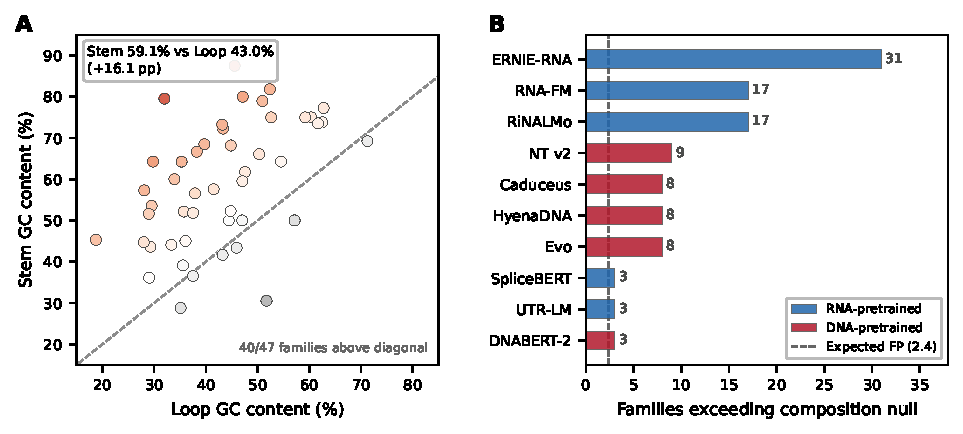
\includegraphics[width=\textwidth]{../figures_v24/figure2_composition_v24b.pdf}
\caption{Composition confound. (A)~Stem GC content exceeds loop GC content
in \panelGCEnriched{} of \panelGCScored{} families (mean stem GC
\panelStemGC{}\% against loop GC \panelLoopGC{}\%). (B)~Number
of families per model whose stem--loop sensitivity ratio exceeds the
nucleotide-stratified null at the 95th percentile; dashed line marks the
expected false-positive count under independence
($m \times \alpha = \expectedFalsePositives{}$).
ERNIE-RNA ($\exceedErnieRNA{}$), RiNALMo ($\exceedRiNALMo{}$) and RNA-FM
($\exceedRNAFM{}$) retain the most signal after composition control.}
\label{fig:composition}
\end{figure}


\subsection{Probe validation}
\label{sec:probe-validation}

Five of the eight models this readout resolves score at their own chance rate
at Rung~3 once the layer is chosen out of sample, which admits two
readings the panel cannot separate, because every arm in it is a model under test.
We therefore run the Rung 3 procedure unchanged on two constructed embeddings
whose answer is fixed in advance. In the oracle, each position's representation
is a function of its own nucleotide and its partner's; in the local control, of
its own nucleotide and its two sequence neighbors.

The oracle reaches per-pair precision $1.000$ against a derangement chance rate
of $0.051$, and a matched-decoy rate of $1.000$. The local control reaches
precision $0.118$ against a chance rate of $0.164$, and a matched-decoy rate of
$0.499$. Precision and chance are over the $\chanceRateN{}$ families of the
Rung~3 analysis set and the matched-decoy rates over the 17 families that admit
the comparison, with the statistic, the null and the code path of every model
row.

The procedure therefore detects a partner-localized representation and rejects
a neighbor-only representation. A model at its chance rate shows no
partner-localized perturbation response detectable by this assay, which does not
establish that no pairing information is decodable from it by another readout.

Per-pair precision has a limit that these two constructions do not expose. A
response that moves every position carrying the partner's nucleotide equally,
with no knowledge of which of them is the partner, also places the partner above
its two stem neighbors whenever those neighbors carry a different nucleotide.
Scored pair by pair over the panel, such a complementarity-only response reaches
Rung~3 precision $87/190 = 0.458$. Rung~3 precision above a model's chance rate
therefore does not by itself show that the response is to the partner, and the
matched-decoy test of Section~\ref{sec:decoy-results} is built to separate the
two.

\subsection{Partner specificity (Rung 3)}
\label{sec:ps-results}

\begin{table}[htbp]
\centering
\caption{Mutation sensitivity across ten models on the repaired panel
($N = \panelN{}$ Rfam families). Bootstrap 95\% CIs on the mean ratio
resample per-family ratios ($B = 10{,}000$).
At $\alpha = 0.05$ per family, 2.4 of 47
families are expected to exceed the null by chance. Attention $\rho$ is the mean
best-head-best-layer Spearman correlation between symmetrized attention and the
contact map, and is undefined for the three state-space models. Probing $\Delta$
is balanced accuracy minus 0.5. Untrained rows randomize every weight at a fixed
seed and load through the same adapter as the trained row above them.}
\label{tab:rung1}
\small
\begin{tabular}{lrlccc}
\toprule
\textbf{Model} & \textbf{Mean ratio} & \textbf{95\% CI} & \textbf{Fam $>$ null} & \textbf{Attn $\rho$} & \textbf{Probing $\Delta$} \\
\midrule
ERNIE-RNA (86M, RNA)       & 1.276 & [1.22, 1.34] & 31/47 & 0.113 & $+0.183$ \\
RiNALMo (650M, RNA)        & 1.143 & [1.12, 1.17] & 17/47 & 0.107 & $+0.134$ \\
RNA-FM (99M, RNA)          & 1.129 & [1.11, 1.15] & 17/47 & 0.098 & $+0.091$ \\
UTR-LM (1.2M, RNA)         & 1.056 & [1.04, 1.08] & 3/47 & 0.051 & $+0.078$ \\
SpliceBERT (19M, RNA)      & 1.040 & [1.03, 1.05] & 3/47 & 0.054 & $+0.066$ \\
NT~v2 (56M, DNA)           & 1.098 & [1.08, 1.12] & 9/47 & 0.234 & $+0.036$ \\
DNABERT-2 (117M, DNA)      & 0.996 & [0.98, 1.01] & 3/47 & 0.196 & $+0.051$ \\
HyenaDNA (0.45M, DNA)      & 1.160 & [1.12, 1.20] & 8/47 & --- & $+0.077$ \\
Caduceus (7.7M, DNA)       & 1.206 & [1.16, 1.26] & 8/47 & --- & $+0.077$ \\
Evo (7B, DNA)              & 1.458 & [1.30, 1.64] & 8/47 & --- & $+0.052$ \\
\midrule
ERNIE-RNA untrained        & 1.164 & [1.12, 1.21] & 10/47 & 0.085 & $+0.044$ \\
RiNALMo untrained          & 1.156 & [1.13, 1.19] & 10/47 & 0.064 & $+0.077$ \\
RNA-FM untrained           & 1.045 & [1.04, 1.05] & 1/47 & 0.038 & $+0.068$ \\
UTR-LM untrained           & 1.038 & [1.03, 1.04] & 1/47 & 0.054 & $+0.077$ \\
SpliceBERT untrained       & 1.054 & [1.04, 1.07] & 0/47 & 0.032 & $+0.070$ \\
NT~v2 untrained            & 1.015 & [1.01, 1.02] & 5/47 & 0.241 & $+0.025$ \\
DNABERT-2 untrained        & 33.880 & [0.95, 93.92] & 6/47 & 0.153 & $+0.011$ \\
\bottomrule
\end{tabular}
\end{table}


\begin{table}[htbp]
\centering
\caption{Dinucleotide-stratified null across all models on the repaired panel.
``Fam $>$ nuc'' counts families exceeding the nucleotide-stratified null;
``Survive dinuc'' counts how many of those also exceed the
dinucleotide-stratified null, which is computed only where the first-order null
is exceeded. Retention is the second count over the first, and its bootstrap
95\% CI resamples the families in the first.}
\label{tab:rung2}
\small
\begin{tabular}{lrrll}
\toprule
\textbf{Model} & \textbf{Fam $>$ nuc} & \textbf{Survive dinuc} & \textbf{Retention} & \textbf{95\% CI} \\
\midrule
ERNIE-RNA (86M, RNA)       & 31 & 30 & 97\% & [0.90, 1.00] \\
RiNALMo (650M, RNA)        & 17 & 15 & 88\% & [0.71, 1.00] \\
RNA-FM (99M, RNA)          & 17 & 14 & 82\% & [0.65, 1.00] \\
NT~v2 (56M, DNA)           & 9 & 8 & 89\% & [0.67, 1.00] \\
HyenaDNA (0.45M, DNA)      & 8 & 7 & 88\% & [0.62, 1.00] \\
Caduceus (7.7M, DNA)       & 8 & 4 & 50\% & [0.12, 0.88] \\
Evo (7B, DNA)              & 8 & 6 & 75\% & [0.38, 1.00] \\
UTR-LM (1.2M, RNA)         & 3 & 2 & 67\% & [0.00, 1.00] \\
SpliceBERT (19M, RNA)      & 3 & 1 & 33\% & [0.00, 1.00] \\
DNABERT-2 (117M, DNA)      & 3 & 2 & 67\% & [0.00, 1.00] \\
\midrule
ERNIE-RNA untrained        & 10 & 6 & 60\% & [0.30, 0.90] \\
RiNALMo untrained          & 10 & 7 & 70\% & [0.40, 1.00] \\
RNA-FM untrained           & 1 & 1 & 100\% & [1.00, 1.00] \\
UTR-LM untrained           & 1 & 0 & 0\% & [0.00, 0.00] \\
SpliceBERT untrained       & 0 & 0 & --- & --- \\
NT~v2 untrained            & 5 & 4 & 80\% & [0.40, 1.00] \\
DNABERT-2 untrained        & 6 & 4 & 67\% & [0.33, 1.00] \\
\bottomrule
\end{tabular}
\end{table}


\begin{table}[htbp]
\centering
\caption{Perturbation specificity on the repaired panel. 38 of \panelN{} families qualify ($\geq 15$ WC pairs with $\geq 3$ per stem); the two pilot families are quarantined, leaving $N = 36$ confirmatory families. Mean PS is taken over those $N$. Gate counts families passing the stem-versus-loop positive control, and the two null columns are computed among gate-passing families: $>$~null is the primary within-stem derangement null and $>$~cons.\ the conservative variant, reported together because the registration defines both. H3 precision is the mean of per-family partner-is-max fractions. The gate-passing set differs by model, so the null and precision columns are not computed on matched families across rows. Bold rows satisfy H1$_6$ at the repaired gate of 8. NT~v2 and DNABERT-2 qualify on fewer families because their tokenizers resolve short families into too few tokens to perturb.}
\label{tab:rung3}
\small
\begin{tabular}{llrcccc}
\toprule
\textbf{Model} & \textbf{Domain} & \textbf{Mean PS} & \textbf{Gate} & \textbf{$>$ null} & \textbf{$>$ cons.} & \textbf{H3 prec.} \\
\midrule
\textbf{RiNALMo} (650M)      & RNA & \textbf{0.2062} & 33/36 & \textbf{29/33} & 29/33 & 0.859 \\
\textbf{ERNIE-RNA} (86M)     & RNA & \textbf{0.1113} & 34/36 & \textbf{32/34} & 32/34 & 0.885 \\
\textbf{RNA-FM} (99M)        & RNA & \textbf{0.0117} & 31/36 & \textbf{26/31} & 26/31 & 0.717 \\
\textbf{Caduceus} (7.7M)     & DNA & \textbf{0.0039} & 16/36 & \textbf{8/16} & 8/16 & 0.442 \\
Evo (7B)                     & DNA & 0.0017 & 13/36 & 2/13 & 2/13 & 0.376 \\
HyenaDNA (0.45M)             & DNA & 0.0002 & 7/36 & 3/7 & 3/7 & 0.254 \\
SpliceBERT (19M)             & RNA & 0.0002 & 22/36 & 3/22 & 3/22 & 0.290 \\
UTR-LM (1.2M)                & RNA & $8.3 \times 10^{-6}$ & 13/36 & 4/13 & 4/13 & 0.345 \\
NT~v2 (56M)                  & DNA & $-9.7 \times 10^{-5}$ & 34/36 & 6/34 & 6/34 & 0.007 \\
DNABERT-2 (117M)             & DNA & -0.0180 & 24/36 & 4/24 & 4/24 & 0.000 \\
\midrule
ERNIE-RNA untrained          & RNA & $3.4 \times 10^{-9}$ & 13/36 & 11/13 & 11/13 & 0.347 \\
RiNALMo untrained            & RNA & $2.2 \times 10^{-9}$ & 10/36 & 1/10 & 1/10 & 0.191 \\
RNA-FM untrained             & RNA & $2.0 \times 10^{-10}$ & 20/36 & 7/20 & 7/20 & 0.236 \\
UTR-LM untrained             & RNA & $2.3 \times 10^{-9}$ & 28/36 & 10/28 & 10/28 & 0.104 \\
SpliceBERT untrained         & RNA & $6.7 \times 10^{-15}$ & 11/36 & 3/11 & 3/11 & 0.119 \\
NT~v2 untrained              & DNA & $-3.4 \times 10^{-5}$ & 33/36 & 9/33 & 9/33 & 0.000 \\
DNABERT-2 untrained          & DNA & -0.0003 & 19/36 & 2/19 & 2/19 & 0.000 \\
\bottomrule
\end{tabular}
\end{table}


Mutating position $i$ to its complement perturbs its partner $j$ more than it
perturbs $j$'s own stem neighbors in three models. RiNALMo reaches mean
PS $= \psRiNALMo{}$, ERNIE-RNA $\psErnieRNA{}$ and RNA-FM $\psRNAFM{}$
(Table~\ref{tab:rung3}). Over the \chanceRateN{} families whose stems admit a
derangement null, per-pair precision is $\selPerFamilyRiNALMo{}$,
$\selPerFamilyErnieRNA{}$ and $\selPerFamilyRNAFM{}$ against each model's own
chance rate of $\selChanceRiNALMo{}$, $\selChanceErnieRNA{}$ and
$\selChanceRNAFM{}$ (Table~\ref{tab:layer-selection}). The H3 column of
Table~\ref{tab:rung3} averages the same per-family fractions over the
gate-passing families and reads $\hthreeRiNALMo{}$, $\hthreeErnieRNA{}$ and
$\hthreeRNAFM{}$. The remaining five character-tokenized models exceed their own
chance rates by at most $\selExcessCaduceus{}$, reached by Caduceus.

Four models satisfy the registered criterion H1$_6$
(Supplementary Table~S6): mean PS is positive and the count of gate-passing
families above the derangement null meets the registered minimum, under the
primary and the conservative variant, for RiNALMo, ERNIE-RNA, RNA-FM and
Caduceus (\nullCaduceus{} for Caduceus). The count criterion was registered as
7 families at $N = 32$ and is 8 at the repaired $N$. Caduceus's per-pair
precision does not survive layer selection.

None of the five excesses survives the way the layer is chosen. Precision is
read at the layer maximizing mean PS within each family, which is
\chanceRateN{} independent selections, so a model with no partner-specific
response collects the maximum of a noise profile in every family. Choosing one
layer for the whole panel, or choosing it on half the families and reading
precision on the other half over $2{,}000$ splits, moves RiNALMo and ERNIE-RNA
by at most $\selMaxShiftPositive{}$, leaves RNA-FM at $\selHeldOutRNAFM{}$
against a chance rate of $\selChanceHeldOutRNAFM{}$, and puts the five other
character-tokenized models at or below their own chance rates
(Table~\ref{tab:layer-selection}). NT~v2 and DNABERT-2, whose
tokens span several nucleotides, are not in that table; their per-family
precision is $\hthreeNTvTwo{}$ and $\hthreeDNABERTTwo{}$
(Table~\ref{tab:rung3}). Caduceus falls from
$\selPerFamilyCaduceus{}$ to $\selHeldOutCaduceus{}$. Depth does not order the effect: across the \selectionArms{} arms the
correlation between layer count and the drop from per-family to panel selection
is Spearman $\selectionDepthRho{}$ ($p = \selectionDepthP{}$). The held-out
estimate carries no selection at all, and reaches $\selHeldOutRiNALMo{}$ for
RiNALMo ($2.5$th to $97.5$th percentile over splits $\selHeldOutCIRiNALMo{}$),
$\selHeldOutErnieRNA{}$ for ERNIE-RNA ($\selHeldOutCIErnieRNA{}$) and
$\selHeldOutRNAFM{}$ for RNA-FM ($\selHeldOutCIRNAFM{}$).

\begin{table}[htbp]
\centering
\caption{Per-pair precision under three layer choices, each against the model's own within-stem derangement chance rate at the same layer and on the same pairs (in parentheses). Per-family: the layer maximizing mean PS within each family, which is how Table~\ref{tab:rung3} is computed. Panel: one layer maximizing mean PS across all families. Held-out: the layer chosen on half the families and precision reported on the other half, over 2,000 splits; the bracketed interval is the 2.5th to 97.5th percentile over random half-splits and is not a confidence interval over families.}
\label{tab:layer-selection}
\small
\begin{tabular}{@{}lrrrr@{}}
\toprule
\textbf{Model} & \textbf{Layers} & \textbf{Per-family} & \textbf{Panel} & \textbf{Held-out} \\
\midrule
ERNIE-RNA & 13 & 0.888 (0.091) & 0.887 (0.101) & 0.885 (0.102) [0.814, 0.955] \\
RiNALMo & 34 & 0.872 (0.070) & 0.881 (0.077) & 0.879 (0.078) [0.818, 0.938] \\
Caduceus & 17 & 0.340 (0.189) & 0.000 (0.000) & 0.002 (0.002) [0.000, 0.000] \\
RNA-FM & 13 & 0.677 (0.187) & 0.669 (0.185) & 0.669 (0.185) [0.558, 0.779] \\
Evo & 32 & 0.356 (0.326) & 0.314 (0.328) & 0.315 (0.328) [0.231, 0.394] \\
SpliceBERT & 7 & 0.247 (0.228) & 0.203 (0.183) & 0.204 (0.184) [0.152, 0.257] \\
UTR-LM & 7 & 0.246 (0.228) & 0.191 (0.198) & 0.191 (0.198) [0.131, 0.249] \\
HyenaDNA & 4 & 0.138 (0.156) & 0.122 (0.137) & 0.120 (0.136) [0.064, 0.176] \\
ERNIE-RNA untrained & 13 & 0.490 (0.221) & 0.479 (0.245) & 0.479 (0.244) [0.399, 0.558] \\
RiNALMo untrained & 34 & 0.337 (0.241) & 0.158 (0.150) & 0.157 (0.150) [0.108, 0.211] \\
RNA-FM untrained & 13 & 0.235 (0.178) & 0.235 (0.171) & 0.235 (0.170) [0.160, 0.305] \\
SpliceBERT untrained & 7 & 0.171 (0.201) & 0.172 (0.170) & 0.172 (0.170) [0.120, 0.222] \\
UTR-LM untrained & 7 & 0.139 (0.130) & 0.132 (0.120) & 0.131 (0.119) [0.080, 0.181] \\
\bottomrule
\end{tabular}
\end{table}


A chance rate is a property of a model rather than a constant of the comparison.
Measured on the derangement, where the assigned partner is false by
construction, it ranges from $\chanceRateMin{}$ to $\chanceRateMax{}$ across
the panel. Judging
per-pair precision against the exchangeability value of $1/3$ therefore holds
ten models to a threshold none of them has: Caduceus reaches
$\selPerFamilyCaduceus{}$, within $\selVsThirdCaduceus{}$ of $1/3$, and clears
its own rate by $\selExcessCaduceus{}$. Both comparisons are
reported in Table~\ref{tab:rung3}, and RiNALMo, ERNIE-RNA and RNA-FM pass
either.

RiNALMo and ERNIE-RNA concentrate partner specificity late: RiNALMo peaks at layer
$\psPeakRiNALMo{}$ of $\psLayersRiNALMo{}$ in \psPeakCountRiNALMo{} families,
ERNIE-RNA at layer $\psPeakErnieRNA{}$ of $\psLayersErnieRNA{}$ in
\psPeakCountErnieRNA{}. RNA-FM peaks mid-depth, at layer $\psPeakRNAFM{}$ of
$\psLayersRNAFM{}$ in \psPeakCountRNAFM{} families. Among the five resolved
models that do not clear their own chance rates, parameter count orders
nothing: Evo reaches $\psEvo{}$ mean PS with $\paramsOverEvo{}\times$
ERNIE-RNA's parameters, and Caduceus at 7.7M outscores two of the five
RNA-pretrained models on mean PS. The three models whose precision survives
layer selection are all RNA-pretrained, three of five against zero of five. The
registered comparison of mean PS between the RNA-pretrained and DNA-pretrained
models meets its effect-size criterion (rank-biserial $\domainRankBiserial{}$
against a registered threshold of $0.5$) on ten models, a number that does not
resolve the difference ($p = \domainP{}$).

\begin{figure}[htbp]
\centering
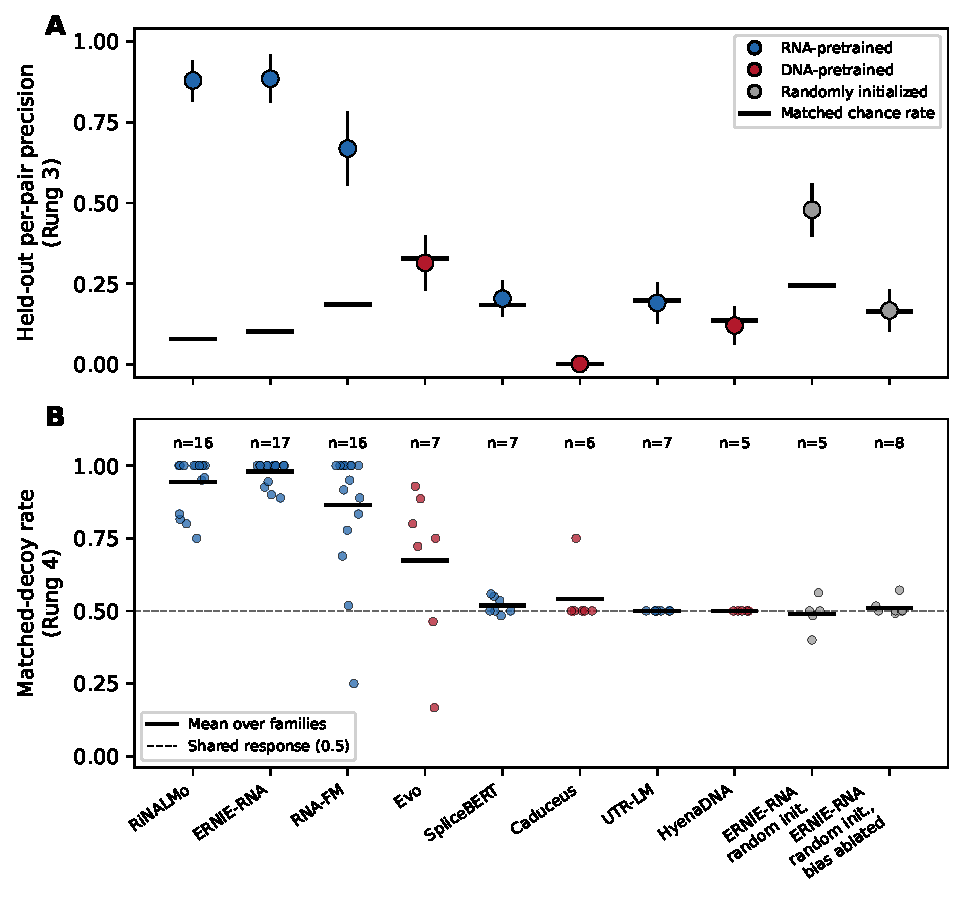
\includegraphics[width=0.85\textwidth]{../figures_v24/figure3_rungs_v24d.pdf}
\caption{Rung~3 and Rung~4 for the eight character-tokenized models and the two
randomly initialized ERNIE-RNA arms. NT~v2 and DNABERT-2 are outside the
registered matched-decoy test because their tokens span several nucleotides.
(A)~Per-pair precision with the layer chosen on half the families and scored
on the other half (points; vertical segments span the 2.5th to 97.5th percentile
over 2{,}000 half-splits) against each arm's matched within-stem derangement
chance rate at that layer (bars). (B)~Matched-decoy rate of
every family the registered audit scored, against all decoys; bars mark the
mean over families, $n$ the number of families contributing, and the dashed
line the value $0.5$ of a response shared by every position carrying the
partner's nucleotide. RiNALMo and ERNIE-RNA lie above $0.5$ in every family.
Randomly initialized ERNIE-RNA exceeds its chance rate in~(A) and sits at
$0.5$ in~(B).}
\label{fig:ps}
\end{figure}


\subsection{Matched-decoy test (Rung 4)}
\label{sec:decoy-results}

Rung~3 compares the partner with its two stem neighbors. A response to the
partner's nucleotide, wherever that nucleotide occurs, passes that comparison
whenever the neighbors carry a different nucleotide
(Section~\ref{sec:probe-validation}), and a response that decays with distance
from the mutated position could favor a partner that happens to lie close. The
matched-decoy test removes both. For each mutated pair $(i, j)$, the decoys are
the partner-side positions of the family's other deep-interior pairs that carry
the same nucleotide as $j$, excluding $j \pm 1$. A family's rate is the mean
over its pairs of the fraction of decoys at which the response is smaller than
at $j$, with ties counted as one half, so a response shared equally by every
position carrying that nucleotide scores exactly $0.5$. The close-decoy
variant keeps only decoys no farther from $i$ than $j$ is, so distance from the
mutation cannot favor the partner. The layer is chosen with the family left
out, and the population is the confirmatory families that pass the model's
stem-versus-loop positive control.

The hypotheses, the statistic, the test and the void rule were registered and
frozen before the run that produced these comparisons
(\texttt{preregistration/complementary\_decoy/PREREG.md}); no matched-decoy
rate had been computed for any model when they were fixed. H1 and H2 state that
the rate exceeds $0.5$ across families for RiNALMo and for ERNIE-RNA, by an
exact one-sided sign test at $\alpha = 0.025$; G1 and G2 state the same against
close decoys and are read only where H1 or H2 holds. A validation gate ran
first: on every family, a constructed response that moves only the partner
must score exactly $1$ and a constructed response that moves every position of
the partner's nucleotide equally must score exactly $0.5$. The gate passed on
all 150 conditions the panel's structure makes available.

\begin{table}[htbp]
\centering
\caption{Matched-decoy test. For each mutated pair, the response at the annotated partner is compared with the response at every other deep-interior paired position of the family that carries the partner's nucleotide (all decoys), and separately with only the decoys no farther from the mutated position than the partner (close decoys). A family's rate is the mean over its pairs of the fraction of decoys the partner exceeds, with ties counted as one half, so $0.5$ is the value of a response shared equally by every such position. Families: the number above, below and at exactly $0.5$, among confirmatory families passing the model's positive control with at least three contributing pairs. The layer is chosen with the family left out. Decision: the registered outcome, from an exact one-sided sign test across families at $\alpha = 0.025$; rows with no decision carry no registered hypothesis. Random init.: every parameter re-initialized. NT~v2 and DNABERT-2 are outside the registered test because their tokens span several nucleotides.}
\label{tab:decoy}
\small
\begin{tabular}{@{}>{\raggedright\arraybackslash}p{3.6cm}rrrrl@{}}
\toprule
 & \multicolumn{2}{c}{\textbf{All decoys}} & \multicolumn{2}{c}{\textbf{Close decoys}} & \\
\cmidrule(lr){2-3}\cmidrule(lr){4-5}
\textbf{Model} & \textbf{Families} & \textbf{Mean rate} & \textbf{Families} & \textbf{Mean rate} & \textbf{Decision} \\
\midrule
RiNALMo & 16/0/0 & 0.944 & 9/0/0 & 0.920 & H1 holds, G1 holds \\
ERNIE-RNA & 17/0/0 & 0.980 & 9/0/0 & 0.954 & H2 holds, G2 holds \\
RNA-FM & 15/1/0 & 0.864 & 7/2/0 & 0.755 &  \\
Evo & 5/2/0 & 0.674 & 2/2/0 & 0.500 &  \\
SpliceBERT & 3/1/3 & 0.518 & 1/2/0 & 0.489 &  \\
Caduceus & 1/0/5 & 0.542 & 0/0/4 & 0.500 &  \\
UTR-LM & 0/0/7 & 0.500 & 0/0/6 & 0.500 &  \\
HyenaDNA & 0/0/5 & 0.500 & 0/0/3 & 0.500 &  \\
\midrule
ERNIE-RNA, random init. & 1/3/1 & 0.489 & 1/1/1 & 0.544 &  \\
ERNIE-RNA, random init., pairing bias ablated & 2/1/5 & 0.510 & 0/4/0 & 0.315 &  \\
\bottomrule
\end{tabular}
\end{table}


All four hypotheses hold and none is void (Table~\ref{tab:decoy}; Figure~\ref{fig:ps}B). RiNALMo's
rate exceeds $0.5$ in \decoyAllAboveRiNALMo{} of \decoyAllFamiliesRiNALMo{}
families (mean $\decoyAllRateRiNALMo{}$, $p = \decoyAllPRiNALMo{}$) and in
\decoyCloseAboveRiNALMo{} of \decoyCloseFamiliesRiNALMo{} against close decoys
(mean $\decoyCloseRateRiNALMo{}$, $p = \decoyClosePRiNALMo{}$). ERNIE-RNA's
exceeds $0.5$ in \decoyAllAboveErnieRNA{} of \decoyAllFamiliesErnieRNA{}
(mean $\decoyAllRateErnieRNA{}$, $p = \decoyAllPErnieRNA{}$) and in
\decoyCloseAboveErnieRNA{} of \decoyCloseFamiliesErnieRNA{}
(mean $\decoyCloseRateErnieRNA{}$, $p = \decoyClosePErnieRNA{}$). In both
models the response to a mutation is localized to the annotated partner
relative to other paired positions carrying the same nucleotide, including
those no farther away. Nucleotide identity does not explain it, and nucleotide
identity combined with distance from the mutation does not explain it either.
The sign test is a test of the median family and not of the mean, and the
comparison is available in \decoyAllFamiliesErnieRNA{} of the \confirmatoryN{}
confirmatory families at most, and in \decoyCloseFamiliesErnieRNA{} for close
decoys, because a family needs at least three pairs with a matched decoy.

The remaining rows carry no registered hypothesis and are reported as
description. RNA-FM passes its positive control in
\decoyPopulationRNAFM{} families and exceeds $0.5$ in \decoyAllAboveRNAFM{} of
\decoyAllFamiliesRNAFM{} (mean $\decoyAllRateRNAFM{}$) and in
\decoyCloseAboveRNAFM{} of \decoyCloseFamiliesRNAFM{} against close decoys
(mean $\decoyCloseRateRNAFM{}$): a response of the same kind as the two
registered models', weaker, and one that the close-decoy comparison would not
have confirmed at the registered threshold. UTR-LM and HyenaDNA tie on every
comparison, because the layer chosen for them is the embedding layer, where a
mutation moves no other position. Caduceus, SpliceBERT and Evo are at or near
$0.5$ on the few families they contribute.

\subsection{The randomly initialized control}
\label{sec:random-init}

Seven models were also run with every parameter re-initialized, holding the
architecture and the tokenizer and destroying the learned weights. On mean PS
the RiNALMo control reaches \psUntrainedRiNALMo{}, against ERNIE-RNA's
\psUntrainedErnieRNA{} and RNA-FM's \psUntrainedRNAFM{}. ERNIE-RNA's
control clears each rung of the ladder. At Rung 1 it exceeds its
composition-preserving null in 10 of $\panelN{}$ families against a chance
expectation of 2.4, retains 6 of those at Rung 2, and reaches per-pair precision
$\selPerFamilyErnieRNAUntrained{}$ at Rung 3 against a chance rate of
$\selChanceErnieRNAUntrained{}$. Judged against the
registered threshold of $1/3$ it passes, at pooled binomial $p = 2.4 \times
10^{-4}$.

The cause is a tensor that randomization does not reach.
\texttt{ErnieRnaModel} holds \texttt{pairwise\_bias\_map}, a
vocabulary-square buffer registered non-persistent, which after the first
forward pass contains six non-zero cells: A--U and U--A at $2.0$, C--G and G--C
at $3.0$, G--U and U--G at $0.8$. Re-initialization iterates a model's
parameters, and a buffer is not a parameter, so the control retains a hardcoded
Watson--Crick and wobble table while its weights are random.

% Written by scripts/evaluate_ernierna_ablation_v24.py. Do not edit.
\begin{table}[htbp]
\centering
\caption{ERNIE-RNA with and without its pairwise bias buffer, trained and
randomly initialized. Per-pair precision is the fraction of deep-interior pairs
whose partner is perturbed more than either of its stem neighbors. Chance is the
same fraction under a within-stem derangement on those pairs, where the assigned
partner is false by construction, and excess is their difference. All four arms
cover the same 35 families. Ablation zeroes
\texttt{pairwise\_bias\_map} and \texttt{pairwise\_bias\_proj} and sets the
rebuild guard, without which the first forward pass restores the buffer.}
\label{tab:ablation}
\begin{tabular}{@{}lccc@{}}
\toprule
\textbf{Arm} & \textbf{Precision} & \textbf{Chance} & \textbf{Excess} \\
\midrule
Trained, bias intact         & 0.888 & 0.091 & $+0.797$ \\
Trained, bias ablated        & 0.842 & 0.108 & $+0.735$ \\
Random-init, bias intact     & 0.490 & 0.221 & $+0.269$ \\
Random-init, bias ablated    & 0.281 & 0.245 & $+0.036$ \\
\bottomrule
\end{tabular}
\end{table}


Ablating that table and the projection above it, with the model's rebuild guard
set so the first forward pass cannot restore it, separates the two arms
(Table~\ref{tab:ablation}).
Writing excess as precision minus that arm's own
chance rate, the randomly initialized model falls from
$\ablationExcessUntrainedIntact{}$ to $\ablationExcessUntrainedAblated{}$, a
loss of $\ablationControlLoss{}$ (95\% CI $\ablationControlLossCI{}$), while the
trained model falls from $\ablationExcessTrainedIntact{}$ to
$\ablationExcessTrainedAblated{}$. The difference between those losses is
$\ablationLossDifference{}$ ($\ablationLossDifferenceCI{}$), and the trained
model's remaining excess is $\ablationTrainedRemaining{}$
($\ablationTrainedRemainingCI{}$), all over $\ablationN{}$ families with
$\bootstrapB{}$ resamples. The three hypotheses of the ablation's registration
hold. Its predictions and criteria were fixed before either ablated arm was
first computed; the chance rate here is the matched one
(Section~\ref{sec:stats}).

The matched-decoy test separates the control from the trained model where
per-pair precision does not. The randomly initialized ERNIE-RNA sits at
$\decoyAllRateErnieRNAUntrained{}$ against all decoys, with
\decoyAllAboveErnieRNAUntrained{} families above $0.5$,
\decoyAllBelowErnieRNAUntrained{} below and \decoyAllAtHalfErnieRNAUntrained{}
at it, and at $\decoyAllRateErnieRNAUntrainedAblated{}$ with the table ablated
(Table~\ref{tab:decoy}). The hardcoded table raises the response at every
position carrying the partner's nucleotide, which is enough to lift the partner
above its stem neighbors and is not a response to the partner.

Across the other nine models no buffer encodes anything about base pairing;
the rest carry position indices, rotary frequencies, or all-zero token-type
vectors, which survive randomization and record where a nucleotide sits. The
RiNALMo control sits $\selExcessRiNALMoUntrained{}$ above its own chance rate
when the layer is chosen within each family, and that excess comes from the
layer choice: with the layer chosen on held-out families it reaches
$\selHeldOutRiNALMoUntrained{}$ against a chance rate of
$\selChanceHeldOutRiNALMoUntrained{}$. The RNA-FM control reaches
$\selHeldOutRNAFMUntrained{}$ against $\selChanceHeldOutRNAFMUntrained{}$
under the same selection, with an interval over splits of
$\selHeldOutCIRNAFMUntrained{}$ that contains its chance rate.

\subsection{Multi-sequence replication}
\label{sec:multiseq-results}

Each family is represented in the panel by one curated sequence, so a ratio
could be a property of that sequence rather than of the family. We therefore
score 3--5 members of each family's Rfam seed alignment, \multiseqN{} sequences
over \multiseqFamilies{} families, and measure the within-family coefficient of
variation of the stem--loop ratio. Every model is scored on the same set.

\begin{table}[htbp]
\centering
\caption{Multi-sequence replication. Each family contributes 3--5 members of its Rfam seed alignment, giving 230 sequences over 47 families, and every model is scored on the same set. CV is the within-family coefficient of variation of the stem--loop sensitivity ratio, averaged over families. Three sequences carrying IUPAC ambiguity codes are excluded for every model (\texttt{Corona\_5UTR\_seq0}, \texttt{Corona\_5UTR\_seq1}, \texttt{Corona\_5UTR\_seq3}). A low CV means the ratio is a property of the family rather than of the one curated representative.}
\label{tab:multiseq}
\begin{tabular}{@{}lrrr@{}}
\toprule
\textbf{Model} & \textbf{Mean ratio} & \textbf{Mean CV} & \textbf{Median CV} \\
\midrule
Evo & 1.334 & 0.180 & 0.155 \\
ERNIE-RNA & 1.256 & 0.059 & 0.057 \\
Caduceus & 1.210 & 0.060 & 0.046 \\
HyenaDNA & 1.171 & 0.093 & 0.088 \\
RiNALMo & 1.135 & 0.036 & 0.032 \\
RNA-FM & 1.118 & 0.034 & 0.031 \\
NT~v2 & 1.091 & 0.044 & 0.039 \\
UTR-LM & 1.059 & 0.025 & 0.023 \\
SpliceBERT & 1.049 & 0.027 & 0.023 \\
DNABERT-2 & 0.997 & 0.054 & 0.049 \\
\bottomrule
\end{tabular}
\end{table}


Nine of the ten models have a mean within-family CV below $0.10$
(Table~\ref{tab:multiseq}). For those models the ratio is a property of the
family and the single curated representative is a fair stand-in for it. The
three models that clear Rung~3 are at $\cvRiNALMo{}$ (RiNALMo),
$\cvErnieRNA{}$ (ERNIE-RNA) and $\cvRNAFM{}$ (RNA-FM).

Evo is the exception, at $\cvEvo{}$. It has the panel's largest raw ratio and
exceeds the nucleotide-stratified null in $\exceedEvo{}$ families
(Section~\ref{sec:composition-results}). A ratio that varies this much between
members of one family, and is largely absorbed by a composition null, is
what a sequence-composition response looks like rather than a structural one.

\subsection{Robustness analyses}
\label{sec:robustness}

Under the dinucleotide-stratified null ERNIE-RNA retains \retainErnieRNA{} of
its Rung~1 families, RiNALMo \retainRiNALMo{} and RNA-FM \retainRNAFM{}
(Table~\ref{tab:rung2}). Replacing
mean aggregation with the median moves the PS estimate by
\robustMedianChangeRiNALMo{} for RiNALMo, \robustMedianChangeErnieRNA{} for
ERNIE-RNA and \robustMedianChangeRNAFM{} for RNA-FM, whose PS is concentrated in
a minority of families; the order of the three is unchanged. Reading PS at the
last layer rather than each family's best changes RiNALMo by
\robustLastLayerChangeRiNALMo{} and ERNIE-RNA by
\robustLastLayerChangeErnieRNA{}, because both peak at or beside their final
layer, and RNA-FM by \robustLastLayerChangeRNAFM{}, because it peaks mid-depth
(Section~\ref{sec:ps-results}).
A transversion control (\transversionAlphabet{}, substitutions that disrupt
pairing without being complement swaps) reproduces the Watson--Crick ratios
across all ten models, with the widest deviation \transversionWidestDeviation{}
at \transversionWidest{} and seven models inside $2.2$\%
(Supplementary Table~S5). The stem--loop contrast is not an artifact of
the substitution alphabet. \controlsNearZero{} of the \controlsTotal{} randomized-weight
controls produce $|\text{mean PS}| < 10^{-8}$. The two that do not are the
multi-nucleotide tokenizers, NT~v2 at $\controlMeanPSNTvTwo{}$ and DNABERT-2 at
$\controlMeanPSDNABERTTwo{}$.
DNABERT-2 is not resolved at Rung~3. Two forward passes of one unmutated
sequence give it a mean PS of $\noopMeanPSDNABERTTwo{}$ over the \confirmatoryN{} confirmatory
families, against $\noopMutatedPSDNABERTTwo{}$ for the mutated comparison, so its row in
Table~\ref{tab:rung3} is not resolved above its no-op floor; every other arm
returns a no-op PS below $10^{-16}$ in every family.
The two Rung 3 statistics disagree on these controls: ERNIE-RNA's has mean PS
$\controlMeanPSErnieRNA{}$ and per-pair precision
$\selPerFamilyErnieRNAUntrained{}$, so a mean PS at zero does
not place a control at chance.

The attention--contact channel, the transversion control, the registered
hypotheses and the run provenance are Supplementary Tables~S4--S7; per-family
ratios, gate outcomes and partner specificity are Supplementary Tables~S2
and~S3.


Twenty hypotheses registered across four protocols before the matched-decoy
registration produce eleven confirmations and nine failures on this panel
(Supplementary Table~S6). The registered prediction that RNA-pretrained models
would exceed DNA-pretrained models on partner specificity meets its effect-size
criterion (Section~\ref{sec:ps-results}).

\subsection{Covariation versus geometry}
\label{sec:covariation-results}

Partner specificity could reflect sequence covariation rather than
learned geometric pairing. Compensatory mutations that maintain base
pairing are overrepresented in evolutionary RNA alignments; a model
trained on such sequences might predict that mutating one position
perturbs its covarying partner without encoding the physical mechanism
of pairing.

To test this, each panel family was regenerated \synPerFamily{} times with its
dot-bracket structure preserved exactly and its nucleotides reassigned---uniform
Watson--Crick pairs at paired positions, uniform elsewhere---giving \synN{}
sequences that share structure with their natural counterparts and carry no
evolutionary covariation. All ten models were run on them
(Table~\ref{tab:synthetic}).

\begin{table}[htbp]
\centering
\caption{Partner specificity on natural and synthetic sequences. Synthetic sequences keep each family's dot-bracket structure and reassign its nucleotides -- uniform Watson--Crick pairs at paired positions, uniform elsewhere -- five per family, so they carry no evolutionary covariation. Excess is per-pair precision minus that arm's own within-stem derangement chance rate, over 35 natural and 195 synthetic sequences. Mean PS falls further than excess precision does, because PS is a magnitude and the synthetic sequences are less structured in composition.}
\label{tab:synthetic}
\small
\begin{tabular}{@{}lrrrrr@{}}
\toprule
 & \multicolumn{2}{c}{\textbf{Mean PS}} & \multicolumn{3}{c}{\textbf{Excess precision over own chance}} \\
\cmidrule(lr){2-3}\cmidrule(lr){4-6}
\textbf{Model} & \textbf{Natural} & \textbf{Synthetic} & \textbf{Natural} & \textbf{Synthetic} & \textbf{Retained} \\
\midrule
RiNALMo (650M) & 0.2062 & 0.0919 & +0.770 & +0.582 & 76\% \\
ERNIE-RNA (86M) & 0.1113 & 0.0415 & +0.764 & +0.574 & 75\% \\
Caduceus (7.7M) & 0.0039 & 0.0036 & +0.122 & +0.058 & 48\% \\
Evo (7B) & 0.0017 & 0.0013 & +0.040 & +0.016 & --- \\
HyenaDNA (0.45M) & $2.4 \times 10^{-4}$ & $1.5 \times 10^{-4}$ & -0.010 & +0.005 & --- \\
SpliceBERT (19M) & $2.2 \times 10^{-4}$ & $2.3 \times 10^{-4}$ & +0.009 & +0.057 & --- \\
RNA-FM (99M) & 0.0117 & 0.0065 & +0.470 & +0.291 & 62\% \\
UTR-LM (1.2M) & $8.3 \times 10^{-6}$ & $1.5 \times 10^{-5}$ & +0.016 & +0.035 & --- \\
NT~v2 (56M) & $-9.7 \times 10^{-5}$ & $-2.1 \times 10^{-4}$ & +0.000 & -0.001 & --- \\
DNABERT-2 (117M) & -0.0180 & -0.0204 & +0.000 & +0.000 & --- \\
\bottomrule
\end{tabular}
\end{table}


Mean PS falls by \synPSDropErnieRNA{} for ERNIE-RNA, to \synPSErnieRNA{}, and
by \synPSDropRiNALMo{} for RiNALMo, to \synPSRiNALMo{}. Per-pair precision
measured against each arm's own chance rate falls by a quarter: ERNIE-RNA's
excess goes from \natExcessErnieRNA{} to \synExcessErnieRNA{} and RiNALMo's
from \natExcessRiNALMo{} to \synExcessRiNALMo{}, retaining
\synRetainedErnieRNA{} and \synRetainedRiNALMo{}. The two statistics answer
different questions on these sequences. Mean PS is a magnitude, and synthetic
sequences have flatter composition, so every perturbation is smaller. Per-pair
precision asks whether a mutated position's partner moves more than that
partner's neighbors, which is what Rung 3 tests, and three quarters of it
survives on sequences with no covariation at all. RNA-FM retains a smaller
share of a smaller excess (Table~\ref{tab:synthetic}). Those sequences also destroy
natural sequence context, so the quarter that is lost is an upper bound on the
covariation contribution and the three quarters that remain are a lower bound
on the rest.

As an independent check, we computed mutual information (MI) between
paired positions from the Rfam seed alignments of \miFamilies{} panel families.
MI separates paired from unpaired positions (mean MI $= \miPaired$ against
$\miUnpaired$; Wilcoxon $p = \miWilcoxonP$), confirming that evolutionary
covariation is detectable in the alignments. Per-family mean MI is
weakly associated with model PS (RiNALMo: $\rho = \miRhoRiNALMo$,
$p = \miPRiNALMo$; ERNIE-RNA: $\rho = \miRhoERNIERNA$, $p = \miPERNIERNA$;
RNA-FM: $\rho = \miRhoRNAFM$, $p = \miPRNAFM$; $n = \miNRiNALMo$). None of the
three associations is significant at $0.05$, and with \miNRiNALMo{} families the
comparison cannot exclude a moderate association.
The synthetic sequences above carry the bound on the covariation contribution.


\subsection{HTT case study}
\label{sec:htt-results}

The CAG repeat region in huntingtin exon~1 folds into hairpins
\citep{demezer2011mutant}, and expanded repeat tracts form more stable
structures than normal-length ones \citep{krzyzosiak2012triplet}. We evaluated
five HTT exon~1 fragments (NM\_002111.7) with CAG repeat counts of 17, 21, 36,
40 and 60, folded with ViennaRNA RNAfold \citep{lorenz2011viennarna}, through
the panel's own stages.

\begin{table}[htbp]
\centering
\caption{Five HTT exon~1 fragments with CAG repeat counts 17, 21, 36, 40 and 60, folded with ViennaRNA. Ratio and $>$~null are stem--loop mutation sensitivity against the nucleotide-stratified null; Attn~$\rho$ is the mean Spearman correlation between self-attention and the contact map, absent for the state-space models; Probing is linear-probe accuracy for stem-versus-loop classification. CAG60 is cosine distance from the CAG17 fragment, at the final layer and at the embedding layer. The repeat region contains no U, so a linear probe has an extreme composition bias available to it, and the fragments differ in length, so embedding distance rises with repeat count at the embedding layer for every model ($\rho = +1.00$) before any block has run.}
\label{tab:htt}
\small
\begin{tabular}{@{}lrcrrrr@{}}
\toprule
\textbf{Model} & \textbf{Ratio} & \textbf{$>$ null} & \textbf{Attn $\rho$} & \textbf{Probing} & \textbf{CAG60 last} & \textbf{CAG60 best} \\
\midrule
RiNALMo & 1.031 & 0/5 & 0.054 & 0.983 & 0.0679 & 0.0115 \\
ERNIE-RNA & 1.086 & 0/5 & 0.070 & 0.985 & 0.0229 & 0.2130 \\
RNA-FM & 1.169 & 0/5 & 0.043 & 0.972 & 0.0148 & 0.0177 \\
UTR-LM & 1.151 & 1/5 & 0.039 & 0.971 & 0.0158 & 0.0134 \\
SpliceBERT & 0.996 & 0/5 & 0.036 & 0.975 & 0.0424 & 0.2120 \\
Caduceus & 1.231 & 0/5 & --- & 0.977 & 0.0017 & 0.0070 \\
HyenaDNA & 1.045 & 0/5 & --- & 0.926 & 0.0193 & 0.0249 \\
NT~v2 & 1.012 & 0/5 & 0.124 & 0.623 & 0.0120 & 0.1509 \\
DNABERT-2 & 0.998 & 0/5 & 0.140 & 0.612 & 0.5073 & 0.5073 \\
\bottomrule
\end{tabular}
\end{table}


\httHighProbing{} of \httModels{} models reach linear-probe accuracy above
$0.97$ for stem-versus-loop classification, and \httHighProbingClean{} of those
exceed the composition-preserving null in no more than one of the five
fragments. The repeat region contains only C, A and G, so a linear probe has an
extreme composition bias available to it. Embedding distance from the CAG17
fragment rises with repeat count for all \httMonotone{} models with more than
one layer, and does so at the embedding layer before any block has run, so that
column separates fragments by length and composition and does not rank models
by whether they represent the expansion. High probing accuracy on a predicted
structure coexists here with no composition-controlled signal.


% ============================================================================
% DISCUSSION — 7 paragraphs
% ============================================================================
\section{Discussion}
\label{sec:discussion}

% P1: Primary conclusion + positive result
Composition-matched nulls absorb most of the apparent stem--loop
sensitivity across all ten models. In RiNALMo and ERNIE-RNA the response to a
mutation is localized to the annotated pairing partner, relative to other
paired positions carrying the same nucleotide and to those no farther from the
mutation, in every family that admits the comparison, under a test registered
before it was run. RNA-FM shows a weaker response of the same kind in an
analysis that was not registered. The other five models the readout resolves
show none.

% P2: Why composition matching changes interpretation
The underlying problem is general: whenever a structural annotation
correlates with feature composition, any embedding metric sensitive to
feature identity inherits the correlation. The nucleotide-stratified
permutation null controls for this by breaking the structure--composition
link while preserving nucleotide identity. The matched decoy applies the same
logic one level down, to the positions a response is compared with: a
comparison of the partner against its neighbors rewards a response to the
partner's nucleotide, and a comparison against other positions carrying that
nucleotide does not. The same template applies to any biological structure
correlated with sequence composition.

% P3: Agreement with downstream benchmarks
The two models with registered partner-localized responses, ERNIE-RNA and
RiNALMo, are the leading models of the downstream secondary-structure
benchmark of \citet{zablocki2025benchmarking}, and RNA-FM, the next model in
that benchmark, shows a similar and weaker response here. The two evaluations
measure different things. One scores a predictor trained on the embeddings and
the other asks where a single-nucleotide perturbation lands, with composition,
nucleotide identity and distance controlled. Their agreement links predictive
performance to a partner-localized response that was measured independently of
it.

% P4: Interpret positive models cautiously
RiNALMo and ERNIE-RNA reach partner specificity through different pathways.
ERNIE-RNA injects a base-pairing attention bias, and that bias with random
weights above it lifts per-pair precision to $\selPerFamilyErnieRNAUntrained{}$
against a chance rate of $\selChanceErnieRNAUntrained{}$ while leaving the
matched-decoy rate at $\decoyAllRateErnieRNAUntrained{}$. RiNALMo uses standard
attention with no structural bias and reaches comparable precision at
$\paramsOverRiNALMo{}\times$ the parameters. On synthetic sequences that preserve
structure and destroy covariation (Section~\ref{sec:covariation-results}), both
retain roughly three quarters of their excess over chance. Those sequences also
destroy natural sequence context, so the quarter that is lost bounds the
covariation contribution from above and the three quarters that remain bound
the non-covariation contribution from below. Whether that remainder reflects a
geometric internal model of folding or a statistical regularity of paired
positions is open.

% P5: Randomized-weight controls
A randomized-weight control is meant to hold the architecture and remove what
training put there. It removes what is stored in parameters. ERNIE-RNA's
pairing table is stored in a buffer, so its control keeps a prior about which
nucleotides pair, and a statistic that rewards a response to the partner's
nucleotide reads that prior as structure. The matched-decoy rate does not. A
control of this kind should be checked for state that re-initialization does
not reach, and the statistic it is used with should be one that an
architectural prior cannot satisfy. \citet{sutter2025non} report a randomly
initialized model satisfying a different analysis: an unrestricted alignment
map reaches perfect interchange-intervention accuracy on randomly initialized
language models.

% P5b: What does not predict the result
Scale and architecture family do not predict a partner-localized response. The
three state-space models span mean ratios $\ratioHyenaDNA{}$ to $\ratioEvo{}$
and the seven transformers $\ratioDNABERTTwo{}$ to $\ratioErnieRNA{}$, so the
architecture families overlap on the raw ratio. Evo at 7B
parameters has the largest raw ratio in the panel, high within-family variance,
and no partner-localized response. The three models that respond at the partner
are RNA-pretrained transformers, and the two RNA-pretrained models that do not,
UTR-LM and SpliceBERT, were trained on untranslated regions and on primary
transcripts. Ten models do not separate pretraining corpus from architecture or
size. NT~v2 and DNABERT-2 are not resolved by a nucleotide-level readout, and
their attention--contact correlations do not supply the missing channel: NT~v2
reads $\attnNTvTwo{}$ trained against $\attnUntrainedNTvTwo{}$ randomly
initialized, so its correlation is architectural, and DNABERT-2's trained
excess of $\attnDeltaDNABERTTwo{}$ rests on a model that does not reproduce
itself between runs (Supplementary Table~S4).

% P6: Limitations
% (Updated to reference covariation results in Section 2.5)
\paragraph{Limitations.}
Every test here perturbs the input sequence and reads a representation. A
positive result locates a response at the partner; it does not identify the
attention heads or other components that produce it, and it is not a
mechanistic account of how a model represents pairing. Interventions on
internal activations, as \citet{lu2026two} apply to protein structure models,
are the route to such an account. The readout is one
operational test. A model at its chance rate shows no
partner-localized response to a complement swap; that does not establish that
no pairing information can be decoded from it by another method. The
structures are Rfam consensus structures and not experimentally determined
structures of the sequences scored. The matched-decoy comparison needs
families with several same-nucleotide pairs deep in their stems, which leaves
\decoyAllFamiliesErnieRNA{} of the \confirmatoryN{} confirmatory families at
most, and \decoyCloseFamiliesErnieRNA{} for close decoys. RNA-FM's
matched-decoy result is descriptive: it had no registered hypothesis. The
complement-swap metric does not test tertiary contacts, pseudoknots or
non-canonical pairs. The synthetic covariation control
(Section~\ref{sec:covariation-results}) removes covariation and natural
sequence context together, so the quarter of the excess it costs is an upper
bound on what covariation contributes. HTT structures are RNAfold predictions.
Pretraining-set overlap with the panel cannot be fully reconstructed.
Multi-nucleotide tokenization leaves NT~v2 and DNABERT-2 unresolved.

\paragraph{Practical recommendations.}
A claim that a representation encodes RNA secondary structure should report
stem--loop sensitivity beside a nucleotide-stratified null, so that composition
sensitivity and structure awareness can be told apart. A claim about pairing
should compare the response at the partner with the response at other
positions carrying the partner's nucleotide, and should say how far those
positions are from the perturbation. Chance should be measured for each model,
at the layer and on the pairs the statistic is read on. The read-out layer
should be chosen on families that do not report the number. A randomized-weight
control should be checked for buffers and other state that re-initialization
leaves in place. For multi-nucleotide tokenizers, the mapping from tokens to
positions should be stated, and a nucleotide-level hypothesis that the mapping
cannot resolve should be reported as unresolved.

% ============================================================================
% MATERIALS AND METHODS (after Discussion per RNA journal format)
% ============================================================================
\section{Materials and Methods}
\label{sec:methods}

\subsection{Benchmark construction}
\label{sec:benchmark}

We evaluate \panelN{} Rfam~14.10 families \citep{kalvari2021rfam} spanning ribozymes, riboswitches, snRNAs,
cis-regulatory elements, miRNA precursors, CRISPR repeats, and other ncRNAs.
Positions are labeled stem or loop from consensus dot-bracket annotation.
Minimum inclusion criteria: $\geq 20$~nt, $\geq 5$ stem and $\geq 5$ loop
positions. Pseudoknots, noncanonical pairs, and gap positions are excluded.

All structures are consensus secondary structures from Rfam seed alignments;
none are experimentally determined crystal or cryo-EM structures. Pretraining
data overlap cannot be fully reconstructed for all models. The full family
list with accessions appears in Supplementary Table~S1.

\subsection{Models and controls}
\label{sec:models}

\begin{table}[htbp]
\centering
\caption{Models evaluated.}
\label{tab:models}
\begin{tabular}{@{}llrll@{}}
\toprule
\textbf{Model} & \textbf{Domain} & \textbf{Params} & \textbf{Architecture} & \textbf{Tokenization} \\
\midrule
RNA-FM \citep{rnafm}                    & RNA & 99M  & Transformer           & Character \\
RiNALMo \citep{rinalmo}                 & RNA & 650M & Transformer           & Character \\
ERNIE-RNA \citep{yin2025ernierna}        & RNA & 86M  & Transformer$^\dagger$ & Character \\
SpliceBERT \citep{chen2024splicebert}     & RNA & 19M  & Transformer           & Character \\
UTR-LM \citep{chu2024utrlm}             & RNA & 1.2M & Transformer           & Character \\
NT~v2 \citep{dalla2023nucleotide}        & DNA & 56M  & Transformer           & 6-mer     \\
DNABERT-2 \citep{zhou2024dnabert2}       & DNA & 117M & Transformer           & BPE       \\
Caduceus \citep{schiff2024caduceus}      & DNA & 7.7M & Mamba (SSM)           & Character \\
HyenaDNA \citep{nguyen2024hyenadna}      & DNA & 0.45M & Hyena (SSM)          & Character \\
Evo \citep{nguyen2024evo}                & DNA & 7B   & StripedHyena          & Character \\
\bottomrule
\end{tabular}
\medskip

\small $^\dagger$ERNIE-RNA injects a base-pairing attention bias from the
second layer onward.
\end{table}

We evaluate ten models covering attention, SSM, and hybrid architectures
(Table~\ref{tab:models}): five pretrained on RNA, five on DNA. Each model is
run through the tokenizer and model class its checkpoint is distributed with,
at a pinned revision. Parameter counts are those of the checkpoint each adapter
loads, except DNABERT-2's, which is the authors' figure.
Randomized-weight controls for the seven transformer models reinitialize all
learned parameters (Xavier normal for matrices, $\mathcal{N}(0, 0.02)$
for vectors) while preserving architecture. NT~v2 and DNABERT-2 use
multi-nucleotide tokenization (6-mer and BPE), limiting direct
comparability for position-level metrics.

\subsection{Perturbation tests}
\label{sec:perturbation}

For each annotated position, we swap the nucleotide with its Watson--Crick
complement (A$\leftrightarrow$U, C$\leftrightarrow$G) and measure the cosine
distance between wild-type and mutant embeddings at that position, maximized
over layers. Cosine distance is scale-invariant across architectures. Reading
dependencies between positions from a language model by perturbing its input is
related to the categorical Jacobian of \citet{zhang2024protein}, which extracts
coevolutionary couplings from a protein language model.
For multi-nucleotide tokenization, token-level outputs are mapped to
nucleotide positions by distributing the token embedding equally across
constituent nucleotides.

\paragraph{Nucleotide-stratified null.}
Stem/loop labels are shuffled within each nucleotide type (1{,}000
permutations), preserving nucleotide identity while breaking its structural
label. Layer selection is repeated inside every permutation. A
dinucleotide-stratified extension additionally conditions on the 3' neighbor.

\paragraph{Partner specificity.}
\label{sec:ps-method}
For each Watson--Crick pair $(i, j)$ where $j$ is the annotated partner:
\[
\text{PS}(i,j) = \Delta_j - \max(\Delta_{j-1}, \Delta_{j+1})
\]
where $\Delta_k$ is the cosine distance at position $k$ after the complement
swap at position $i$. Positive PS indicates the model perturbs the true
partner more than its immediate neighbors. Chance for the per-pair comparison
is measured rather than assumed: partner assignments are permuted within each
stem under a derangement (500 derangements), so every position keeps its stem,
its nucleotide and its layer while its assigned partner is false by
construction. Precision is read on pairs at least two positions inside their
stem, and the chance rate is measured on those pairs at the layer the precision
is read at. Measured this way the chance rate ranges from
$\chanceRateMin{}$ to $\chanceRateMax{}$ across the panel.

\paragraph{Matched-decoy test.}
\label{sec:decoy-method}
For a mutated pair $(i, j)$ that lies at least two positions inside its stem,
a decoy is a position $j'$ on the partner side of another such pair of the
same family with the same nucleotide as $j$ and $j' \notin \{j-1, j+1\}$. The
pair's score at a layer is the mean over its decoys of $1$ where
$\Delta_j > \Delta_{j'}$, $0.5$ where they are equal and $0$ otherwise, and a
family's rate is the mean of its pairs' scores. The close-decoy variant keeps
the decoys with $|i - j'| \leq |i - j|$. A family enters a comparison with at
least three contributing pairs. The layer for a family is the one maximizing
mean PS over the model's other families. The population for a model is the
confirmatory families that pass its positive control. The test is an exact
one-sided sign test of the family rates against $0.5$, with families at exactly
$0.5$ dropped, at $\alpha = 0.025$ for each of the two registered models; the
close-decoy guard for a model is read only where its first hypothesis holds. A
hypothesis is void below 14 families (8 for close decoys).

\paragraph{Covariation control.}
To distinguish learned geometric sensitivity from recapitulated evolutionary
covariation, synthetic sequences were generated for each family: dot-bracket
structure preserved exactly, nucleotides assigned randomly (uniform
Watson--Crick pairs at paired positions, uniform random at unpaired). Mutual
information (MI) between paired and unpaired positions was computed from Rfam
seed alignments as an independent covariation measure.

\subsection{Statistical analysis and replication}
\label{sec:stats}

The matched-decoy hypotheses, statistic, layer rule, test, void rule and
validation gate were registered and frozen before the run that produced them
(\texttt{preregistration/complementary\_decoy/PREREG.md}), after the Rung~3
results of this paper had been seen; the registration states what had been
seen. The models other than RiNALMo and ERNIE-RNA carry no hypothesis in it.
Two departures from the earlier registrations are recorded in
\texttt{DEVIATIONS.md}. The Rung~3 chance rate is measured on the pairs
precision is read on, where it was registered over every eligible pair. RNA-FM
is run through its checkpoint's own tokenizer and model class; hypotheses H1,
H6, H6b and H10 of the expanded-panel registration and RNA-FM's rows in the
Phase~6 registration are evaluated on that run.

The biological unit of replication is the RNA family. The primary outcome is
partner specificity (PS); the primary comparison is trained vs.\
randomized-weight PS. A family is \emph{gate-qualifying} for a given model
if mutating a stem position perturbs the other stem positions more than the
loop positions at that family's best layer (paired $t$-test over the family's
eligible pairs, $p < 0.05$). The gate is a separate statistic from the Rung~1
null, so a model's gate count can exceed its Rung~1 count. Mean PS is taken
over the confirmatory families; the counts above the derangement null and the
H3 precision are taken over gate-qualifying families.

To test stability across biological replicates, the Rung~1 stage is repeated on
the seed-alignment members of each panel family: \multiseqN{} sequences across
\multiseqFamilies{} families, 3--5 per family, each scored as its own family and
regrouped afterwards. Within-family coefficient of variation (CV) quantifies
replication stability. Three sequences carrying IUPAC ambiguity codes outside
\texttt{ACGTUN} are excluded for every model, so the comparison is over a common
set.

Family-level bootstrap resampling (10{,}000 iterations, seed 42)
provides 95\% CIs for mean PS and mean sensitivity ratio. For the binary
gate test, each family's ratio is compared to its own 95th-percentile
permutation null; we report the count exceeding this threshold alongside
the expected false-positive count under independence
($m \times \alpha = \panelN{} \times 0.05 = \expectedFalsePositives{}$).
Bonferroni correction
($\alpha / m \approx 0.001$) provides a conservative bound.


% ============================================================================
% DATA AVAILABILITY
% ============================================================================
\section*{Data and Code Availability}

All data, scripts, and pre-registration protocols are available at
\url{https://github.com/elliottower/rna-structure-audit} and archived at
Zenodo (DOI: \href{https://doi.org/10.5281/zenodo.21362717}{10.5281/zenodo.21362717}).

The deposited panel holds one directory per model, each stamped with the commit
and library versions it was computed under, and a manifest naming the run each
file came from. Preregistrations are frozen at a commit hash, deviations are
dated in \texttt{DEVIATIONS.md}, and reported numbers are bound to their runs,
using \texttt{prereg}, \texttt{results} and \texttt{citations}
\citep{tower2026reproducible}.


% ============================================================================
% DECLARATIONS
% ============================================================================
\section*{Acknowledgements}

The author used Claude Code \citep{anthropic2025claude} to assist with
drafting manuscript text and with writing and debugging analysis code.
The author reviewed and verified all outputs, takes full responsibility
for the accuracy and integrity of the work, and confirms that all
hypotheses, preregistered predictions, interpretations, and conclusions
are the author's own.

\paragraph{Ethics approval and consent to participate.}
This study uses exclusively publicly available pretrained model weights
and published RNA sequences. No human subjects or animal subjects were
involved. No ethical approval was required.

\paragraph{Competing interests.} The author declares no competing interests.

\paragraph{Funding.} None. This work was conducted independently.

\paragraph{Author contributions.} E.T.: Conceptualization, Methodology,
Software, Formal analysis, Investigation, Data curation, Writing ---
original draft, Writing --- review \& editing, Visualization.


% ============================================================================
% REFERENCES
% ============================================================================
\bibliographystyle{plainnat}
\bibliography{references}

\end{document}
